% Copyright 2004 by Till Tantau <tantau@users.sourceforge.net>.
%
% In principle, this file can be redistributed and/or modified under
% the terms of the GNU Public License, version 2.
%
% However, this file is supposed to be a template to be modified
% for your own needs. For this reason, if you use this file as a
% template and not specifically distribute it as part of a another
% package/program, I grant the extra permission to freely copy and
% modify this file as you see fit and even to delete this copyright
% notice. 

\documentclass{beamer}
\setbeamercovered{transparent}

\usepackage{color}
\usepackage{amsmath}
\usepackage{subcaption}

\usetheme{Madrid}
\newcommand{\mc}{\mathcal}
\newcommand{\mb}{\mathbf}

\definecolor{lb}{rgb}{0.8,0.8,1}
\newcommand*\MyCitem{\item[\color{lb}{\textbullet}]}

\title[Easy clustering]{When is clustering easy? }

\author[Kushagra, Shrinu]{
A Research Proposal\\
by\\
Shrinu Kushagra\\
\vspace{20pt}Under the supervision of\\
Prof. Shai Ben-David\vspace{20pt}\\
David Cheriton School of Computer Science\\
University of Waterloo
}
%\date{\today}

\AtBeginSubsection[]
{
  \begin{frame}<beamer>
  \frametitle{Outline}
    \tableofcontents[currentsection]
  \end{frame}
}

% Let's get started
\begin{document}

\begin{frame}
  \titlepage
\end{frame}

\begin{frame}{Clustering - Introduction}
	Input: $(\mc X, d)$ and $k$\\
	$\mc X  =\{x_1, \ldots, x_n\}$ and each $ x_i \subseteq \mb M$\\   
	\vspace{1cm}Output: $\mc C = \{C_1, \ldots, C_k\}$\\
	

	\vspace{2cm}

	Partition the input data into \alert{``well-separated''} subsets of \alert{``similar''} instances.
\end{frame}

\begin{frame}{Common approaches to clustering}

	{\color{blue}Linkage-based} \\
	
	\vspace{0.5cm}Input : $(\mc X, d)$
	\vspace{0.2cm}	\begin{block}{}
		Initialize every point in its own cluster.\\
		\vspace{0.41cm}Repeat until only one cluster remains
		\begin{itemize}
			\item Merge the two ``closest" clusters
		\end{itemize}
	\end{block}
	
	\pause
	\vspace{0.5cm}Single-linkage: $$d(C_1, C_2) = \min\{d(x, y): x \in C_1, y \in C_2\}$$
	\vspace{0.5cm}Max-linkage: $$d(C_1, C_2) = \max\{d(x, y): x \in C_1, y \in C_2\}$$
	
\end{frame}

\begin{frame}{An example clustering tree}
	\begin{figure}
	  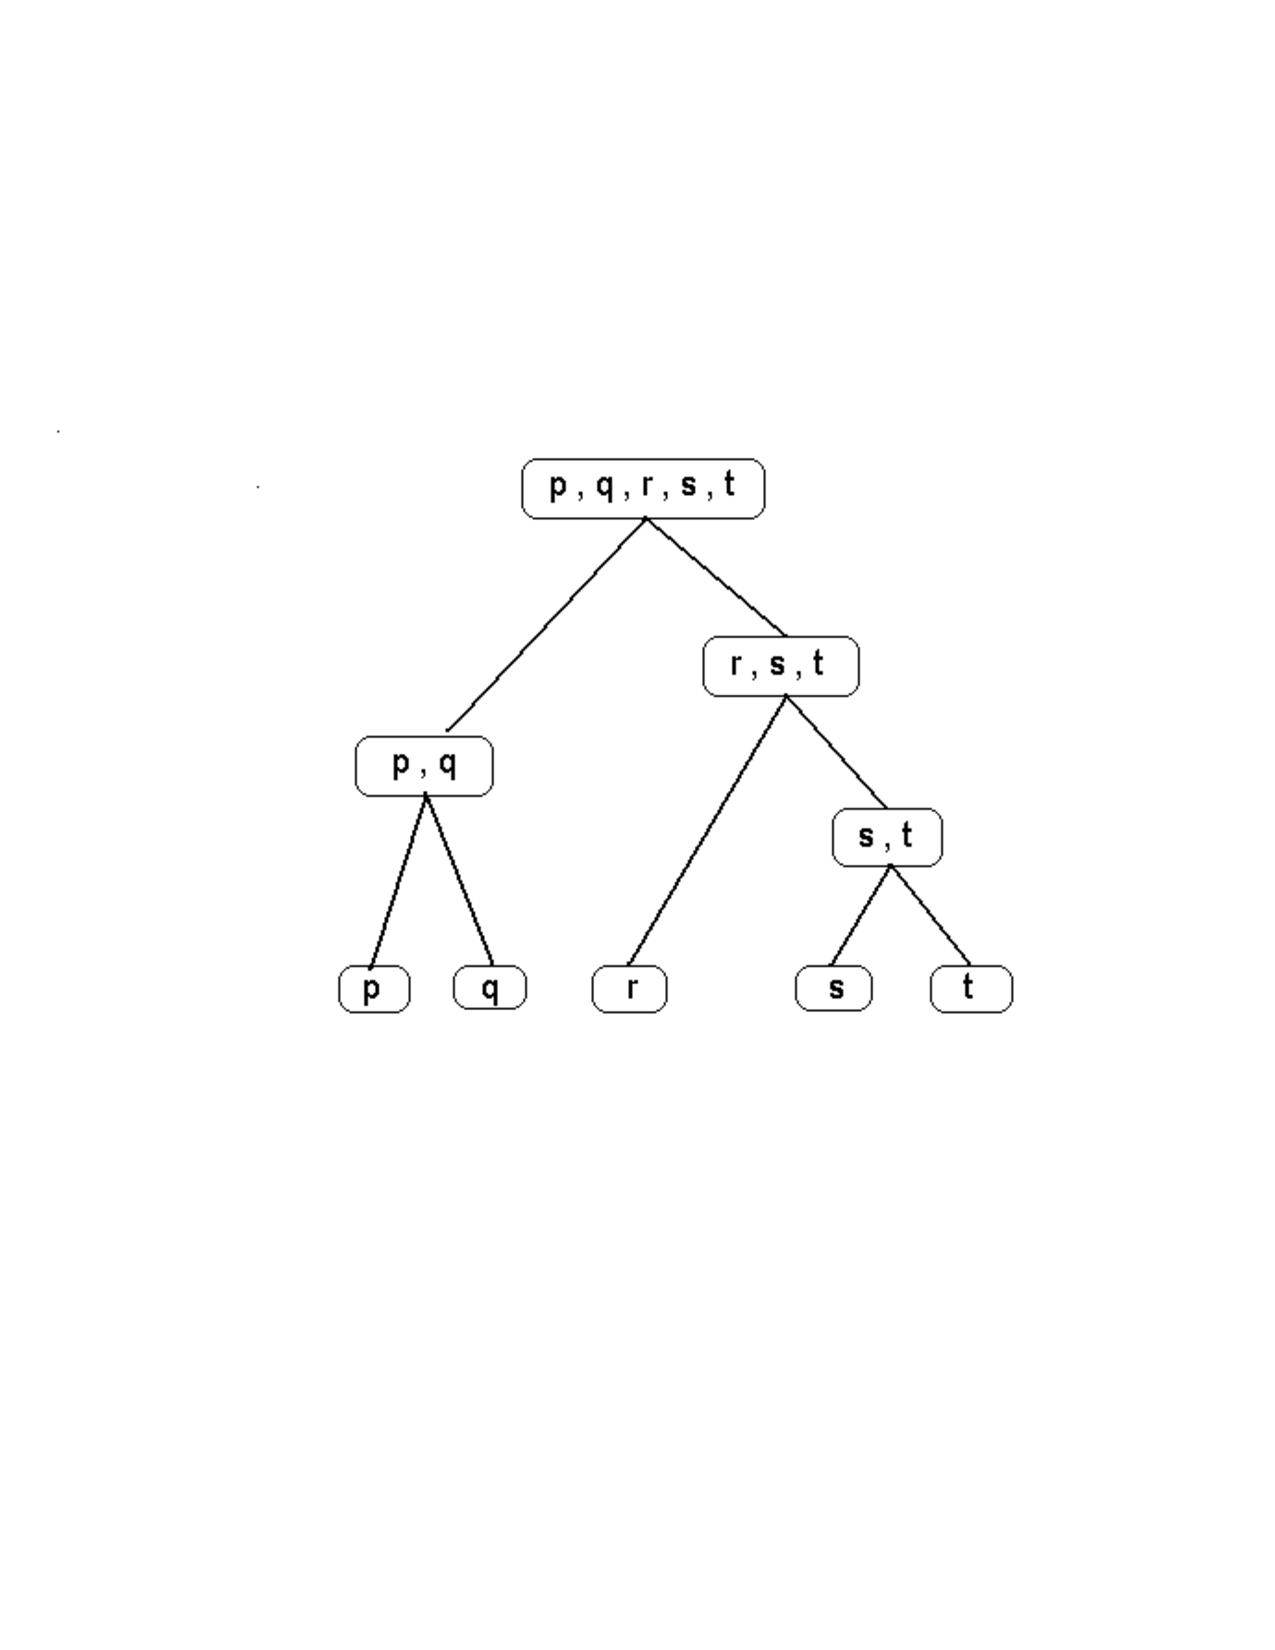
\includegraphics[trim = 50 150 50 200, clip, width=0.8\linewidth]{figures/hier.pdf}
	\end{figure}
\end{frame}

\begin{frame}{Common approaches to clustering}

	{\color{blue}Center-based} \\
	\vspace{0.4cm}Input: $(\mc X, d)$ and $k$\\
	$\mc X  =\{x_1, \ldots, x_n\}$ and each $ x_i \subseteq \mb M$\\   
	
	\vspace{1cm}\alert{Choose} centers $\mu_1, \ldots, \mu_k \in \mb M$\\
	\vspace{0.4cm}	Assign each $x \in \mc X$ to the closest center.
	
	\vspace{1cm}Proper - $\mu_i \in \mc X$\\
	\vspace{0.5cm}Steiner - Unrestricted\\
\end{frame}

\begin{frame}{Common center-based clustering approaches}
	Associate cost with each possible choice of center.\\
	\vspace{0.5cm}Find centers with minimum cost\\

	\vspace{1cm}$K$-means objective$$\min_{\mu_1, \ldots, \mu_k \in \mb M} \sum_{i =1}^k \sum_{x \in C_i} d^2(x, \mu_i)\vspace{1cm}$$
	$K$-median objective $$\min_{\mu_1, \ldots, \mu_k \in \mc X} \sum_{i =1}^k \sum_{x \in C_i} d(x, \mu_i)\vspace{0.5cm}$$
\end{frame}

\begin{frame}{Clustering is not easy}

  {\color{red}Challenges }
  \vspace{0.4cm}
  \vspace{0.3cm}\begin{itemize}
		\vspace{0.3cm}\item Computational Complexity
		\vspace{0.3cm}{\color{lb} \MyCitem  Under-specificity }
	\end{itemize}
\end{frame}

\begin{frame}{Computational hardness of clustering}
	\onslide<1>$K$-means is NP-Hard.
	\begin{itemize}
		\item NP-Hard for $k=2$ \alert{[Dasgupta `08]}
		\vspace{0.4cm}\item NP-Hard in the plane. \alert{[Vattani `09]}
		\vspace{0.4cm}\item NP-Hard to approximate within $(1+\epsilon)$ \alert{[Awasthi et. al `15]}
	\end{itemize} 
	
	\onslide<2>
	\vspace{1cm}$K$-median is NP-Hard \alert{[Megiddo, Supowit `84]}.
	\begin{itemize}
		\vspace{0.4cm}\item $(3+\epsilon)$-approximation is known. \alert{[Arya et. al `04]}
	\end{itemize}
\end{frame}

\begin{frame}{Previous approaches to tackle computational complexity}
	Assume that the optimal clustering is {\color{green}nice}.\\
	\vspace{1.5cm}What is a nice clustering?
	\begin{itemize}
		\vspace{0.4cm}\item $\alpha$-center proximity
		\vspace{0.4cm}\item $\epsilon$-separatedness
	\end{itemize}
\end{frame}

\begin{frame}{Center-proximity}
	Given $(\mc X, d)$ and $k$.\\
	Clustering $\mc C$ induced by centers $\mu_1, \ldots, \mu_k$\\
	
	\begin{center}
	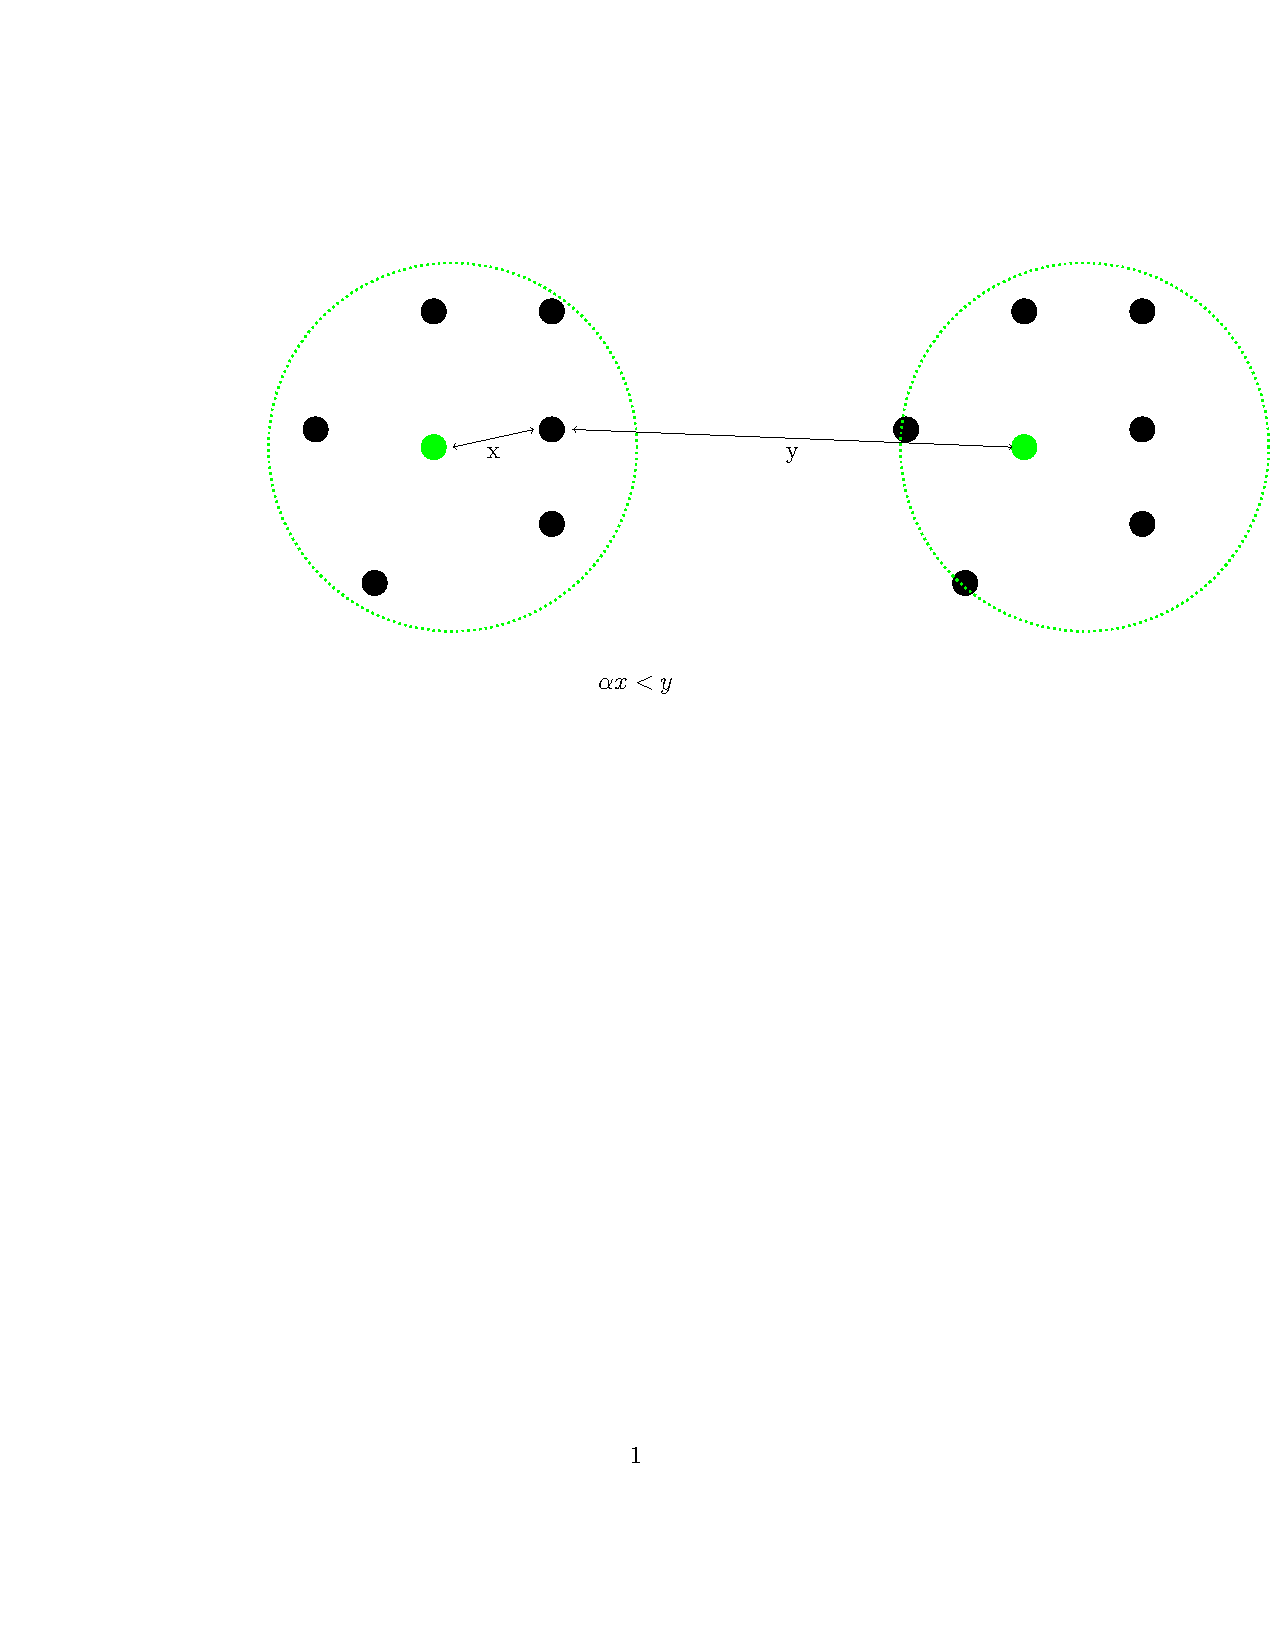
\includegraphics[trim={120 430 0 120},clip,width=0.7\textwidth]{figures/alphacp.pdf}
	\end{center}
	Every point $x$ is closer to its own cluster-center than to other centers\\
	$\alpha$-controls degree of separation.
\end{frame}

\begin{frame}{Formally $\ldots$}
	Given $(\mc X, d)$ and $k$.\\
	\vspace{0.4cm}Clustering $\mc C$ induced by centers $\mu_1, \ldots, \mu_k$\\
	
	\vspace{1cm}\begin{block}{}
		For all $i$, for all $j \neq i$ and for all $x \in C_i$
		$$\alpha d(x, \mu_i) < d(x, \mu_j)$$	
	\end{block}
\end{frame}

\begin{frame}{Clustering under center-proximity}
	Given $(\mc X, d)$ and $k$.\\
	Want to optimize some objective function.\\
	
	\vspace{0.5cm}Assume: Optimal solution satisfies $\alpha$-center proximity.\\
	
	\vspace{1cm}$K$-means objective
	$$\min_{\mu_1, \ldots, \mu_k \in \mb M} \sum_{i =1}^k \sum_{x \in C_i} d^2(x, \mu_i)$$
	\begin{itemize}
		\vspace{0.4cm}\item Efficiently solvable for $\alpha > 2 + \sqrt{3}$ \alert{[Awasthi, Blum, Sheffet `12]}
		\vspace{0.4cm}\item NP-Hard for $\alpha \le 3$ \alert{[Awasthi, Blum, Sheffet `12]}
	\end{itemize}
\end{frame}

\begin{frame}{Clustering under center-proximity}	
	Given $(\mc X, d)$ and $k$.\\
	Want to optimize some objective function.\\
	
	\vspace{0.5cm}Assume: Optimal solution satisfies $\alpha$-center proximity.\\
	
	\vspace{1cm}$K$-median objective
	$$\min_{\mu_1, \ldots, \mu_k \in \mc X} \sum_{i =1}^k \sum_{x \in C_i} d(x, \mu_i)$$
		\begin{itemize}
		\vspace{0.4cm}\item Efficiently solvable for $\alpha > 1 + \sqrt{2}$ \alert{[Balcan, Liang `12]}
		\vspace{0.4cm}\item NP-Hard for $\alpha \le 2$ \alert{[Ben-David, Reyzin `14]}
	\end{itemize}
\end{frame}

\begin{frame}{Issues}
	Assumption on the optimal\\
	\vspace{0.4cm}Can't verify\\
	
	\vspace{1cm}Too strict even for $\alpha = 2$\\
	\begin{center}
	\includegraphics[trim={100 200 100 100},clip,width=0.7\textwidth]{figures/alpha2.pdf}
	\end{center}
\end{frame}

\begin{frame}{Relaxation of center-proximity}
	Given $(\mc X, d)$ and $k$.\\
	\vspace{0.4cm}Clustering $\mc C$ induced by centers $\mu_1, \ldots, \mu_k$
	\vspace{0.5cm}\begin{block}{$(\alpha, \epsilon)$-center proximity}
		There exists $\mc S \subseteq \mc X$ such that 
		\begin{itemize}
			\vspace{0.3cm}\item $|\mc X \setminus \mc S| \le \epsilon n$
			\vspace{0.3cm}\item $\mc C$ restricted to $\mc S$ satisfies $\alpha$-center proximity
		\end{itemize}
	\end{block}
	
	\vspace{0.5cm}If $k$-median optimal satisfies $(2+\sqrt{7}, \epsilon)$-center proximity then 
	\begin{itemize}
		\item Can find $\Big(1 + \frac{8n}{m(\mc C)}\epsilon\Big)$-approximation to the optimal \alert{[Balcan, Liang `12]}.
	\end{itemize}
\end{frame}

\begin{frame}{Other clusterability notions}
	
	{\color{blue}$\epsilon$-separatedness} \alert{[Ostrovsky et. al `12]}\\
	\begin{center}Cost(Opt(k)) $< \epsilon^2$Cost$(Opt(k-1))$\end{center}

	\vspace{0.5cm}Can {\color{blue} explain success} of Lloyd's algorithm \\
	
	
	\vspace{1cm}Algorithm finds a solution of cost atmost $(1+\Theta(\epsilon^2))-Opt$ with probability atleast $(1-\Theta(\epsilon^2))$\\
	
	\vspace{0.5cm} Takes $O(nk + k^3)$ time.
	
\end{frame}

\begin{frame}{Issues}
	\alert{Very strict} separability requirement
	
	\vspace{0.5cm}For $k = 2$, their algorithm succeeds with probability $1 - \frac{20\epsilon^2}{\sqrt{(1-\epsilon^2)(1-101\epsilon^2)}}$ \\

	\vspace{0.5cm}For reasonable guarantee of success $\epsilon^2 < 1/200$\\
	
	\vspace{1cm}This implies that \alert{average radius} is much smaller than separation between two clusters 
	\begin{align*}
		r_i &< \frac{\epsilon}{\sqrt{1-\epsilon^2}} \min_{j \neq i} d(c_i, c_j)\\\\
		\implies 14 r_i &< \min_{j \neq i} d(c_i, c_j) 
	\end{align*}
\end{frame}

\begin{frame}{In conclusion}
Various notions of clusterability.\\
\vspace{1cm}Not easy to verify as they make assumptions on the optimal. \\
\vspace{1cm}Not {\color{blue}realistic}\\
\vspace{1cm}Some can explain popular heuristics. But for unrealistic data. \\

\end{frame}

\begin{frame}{Changing the goal-post}

	Dont care about optimal solution\\
	\vspace{1cm}Happy if the algorithm can output \alert{any (or one) nice} solution\\
	\vspace{1cm}Data set is \alert{nice} if it has a \alert{nice} clustering. 
\end{frame}

\begin{frame}{Realistic clusterability notion}
	Allows for a subset of \alert{background noise}\\
	
	\vspace{1.2cm}Data $\mc X$ consists of 
	\begin{itemize}
	\vspace{0.5cm}
	\item "well clustered" subset $\mc S$ and 
	\vspace{0.5cm}
	\item "unstructured" complement $\mc Y= \mc X \setminus \mc S$,
	\end{itemize}
\end{frame}

\begin{frame}{Our definition: \alert {Sparse Noise}}
	\vspace{0.2cm}Any ball of small radius contains few points from $\mc Y$.
    \begin{figure}
	  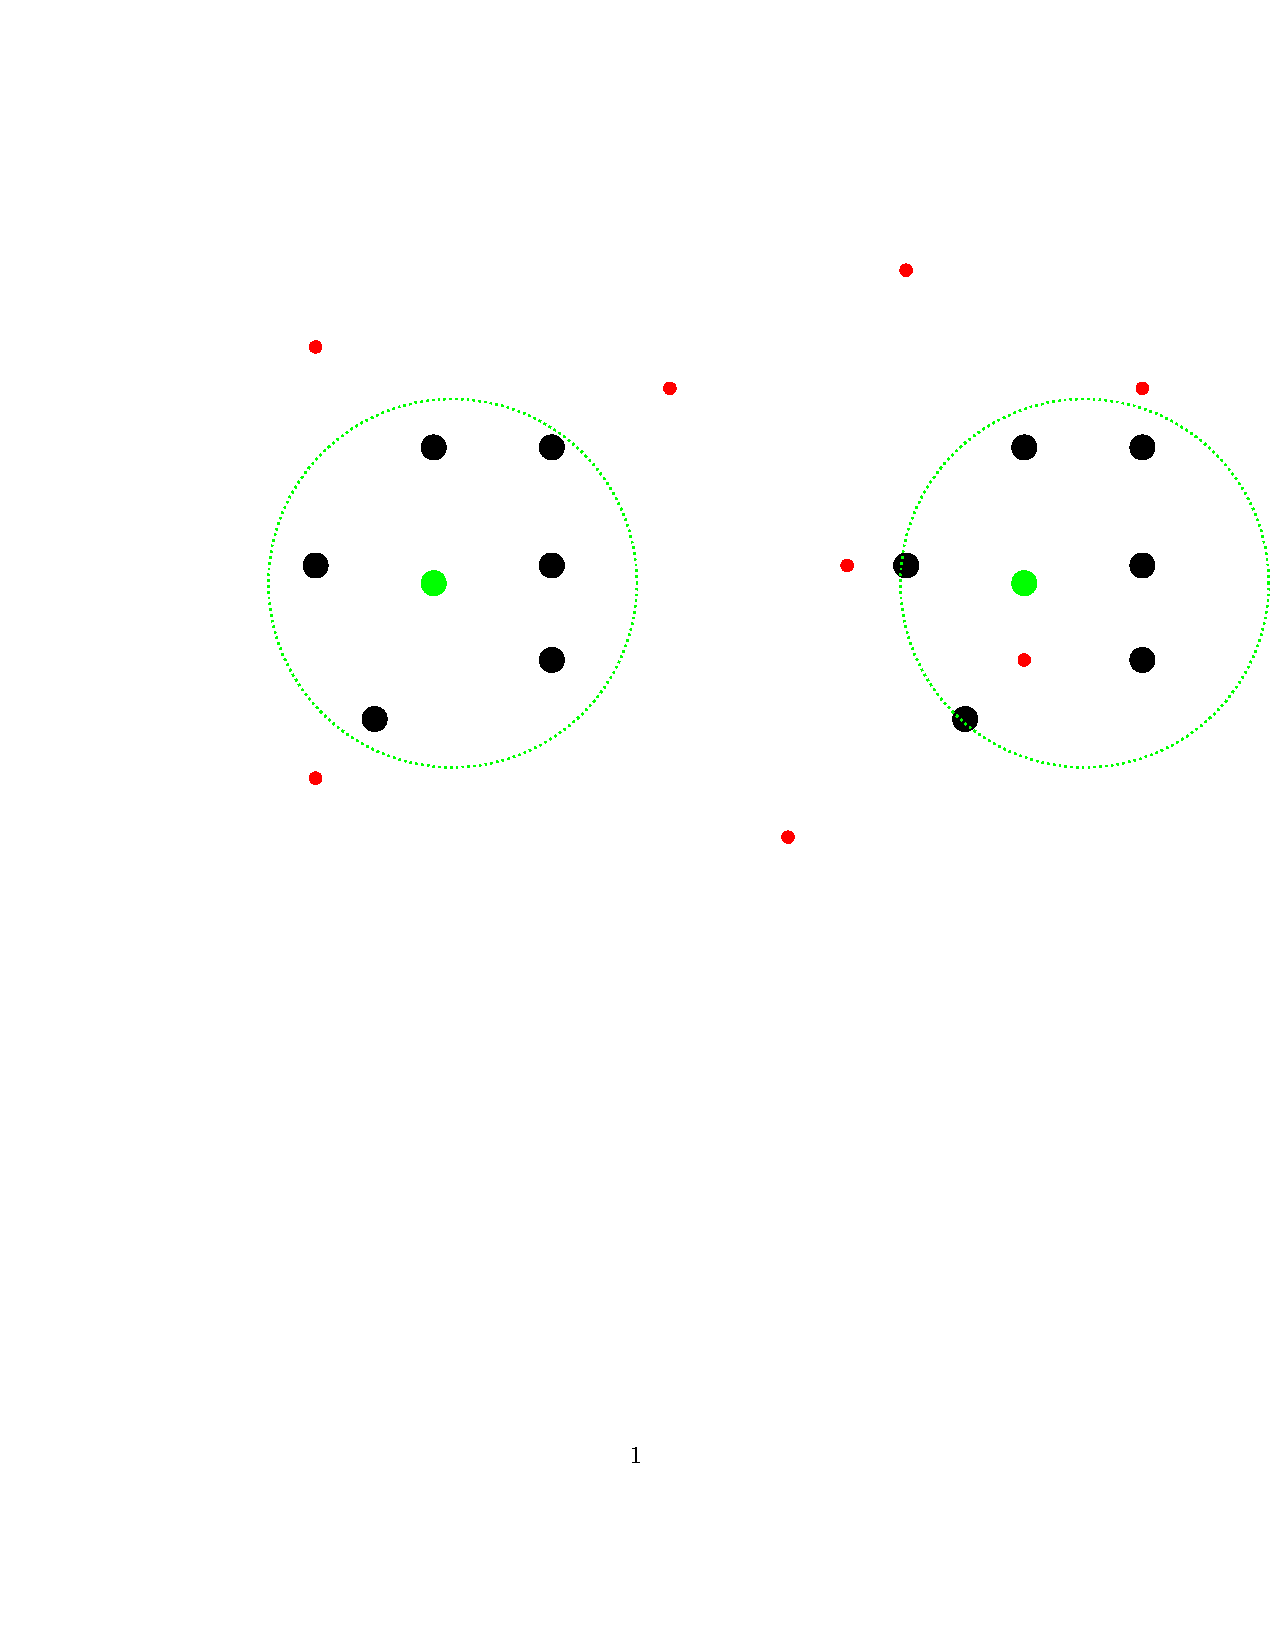
\includegraphics[trim = 100 0 0 100, clip, width=0.8\linewidth]{figures/alphacpnoise.pdf}
   \end{figure}
\end{frame}

\begin{frame}{More formally $\ldots$}

	Given $(\mc X, d)$, a set $\mc S \subseteq \mc X$\\
	\vspace{0.5cm}A clustering $\mc C = \{S_1, \ldots, S_k\}$ of the set $\mc S$ induced by centers $s_1, \ldots, s_k$.

	\vspace{1cm}\begin{block}{$(\alpha, \eta)$-center proximity}
	\vspace{0.5cm} {\bf $\alpha$-center proximity}: For all $x \in S_i$ and $i\neq j$, $$\alpha d(x, s_i) < d(x, s_j)$$
	{\bf $\eta$-sparse noise}: For any ball $B$, 
	$$r(B)\leq \eta \thinspace r(\mc{C}) \implies |B\cap (\mc X\setminus \mc S)| < \frac{m(\mc C)}{2}$$
	\end{block}
\end{frame}

\begin{frame}{Possible justification of sparse noise}
	Data $\mc S$ has nice structure.\\
	\vspace{0.5cm} Noise $\mc N$ is added by a {\color{blue} non-concentrated} distribution.\\
	\pause
	\vspace{1cm} $\mc X = \mc S \cup \mc N$ satisfies the structureless noise definition with high probability.
\end{frame}

\begin{frame}{A high level problem description}

	Design algorithms that get a data set with a metric $(\mc X, d)$ so that
	\vspace{1cm}
	\begin{itemize}
		\item Assuming the data consists of 
		\begin{itemize}
		\vspace{0.5cm}
		\item subset $\mc S$ satisfying $\alpha$-center proximity 
		\vspace{0.5cm}
		\item complement $\mc Y= \mc X \setminus \mc S$ is sparse,
		\end{itemize}

		\vspace{1.5cm}
		\item Outputs a partition $C=(C_1, \ldots C_k)$ that \emph{induces} a good clustering of $\mc S$.
	\end{itemize}
\end{frame}

\begin{frame}{Our Results}
 \alert{Positive results}
 \begin{itemize}
  	\item $\alpha > 4.6$ and noise is sparse\\ 	
	\textcolor{blue}{We construct  in poly time a clustering tree that induces the original nice clustering}.  	
	\begin{figure}
	  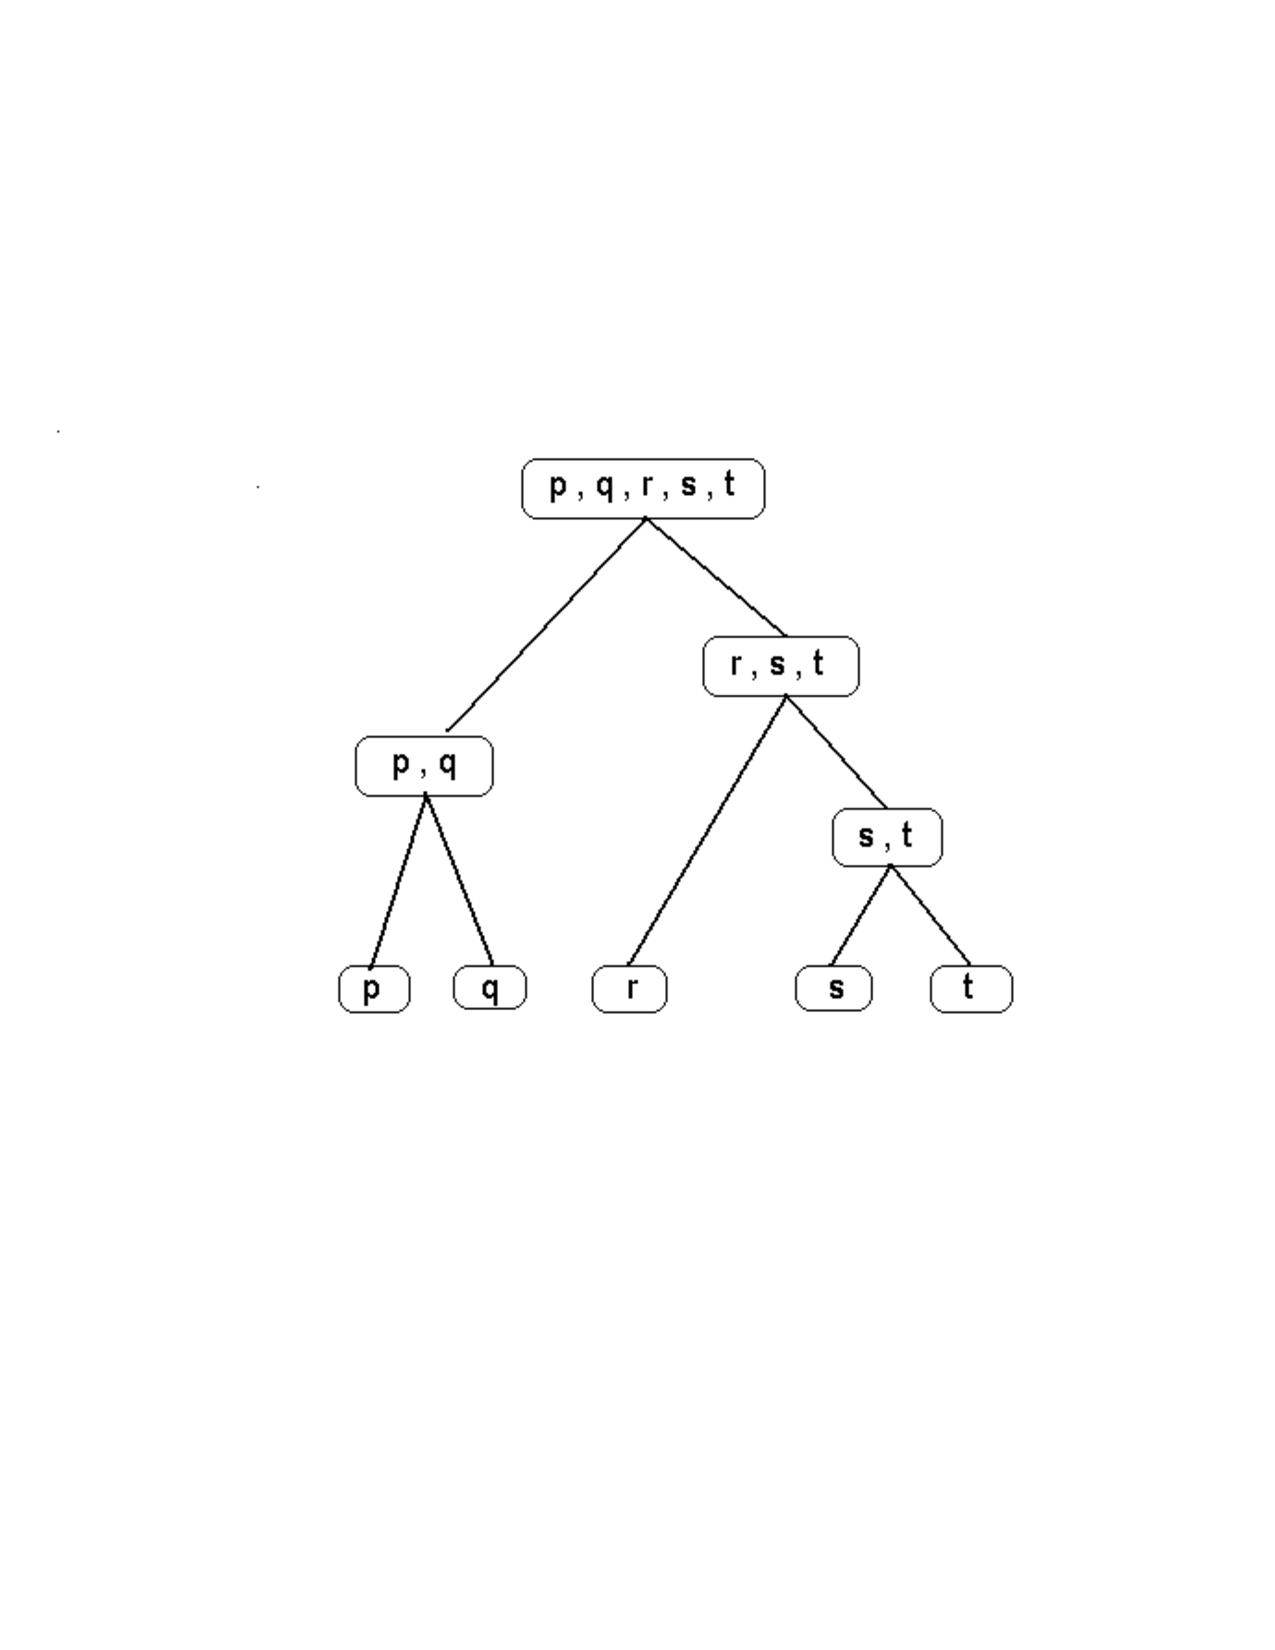
\includegraphics[trim = 50 150 50 200, clip, width=0.8\linewidth]{figures/hier.pdf}
	\end{figure}	  	
  \end{itemize}  
\end{frame}

\begin{frame}{Our Results}
	\alert{Negative results}
  	\begin{itemize}
	  	\vspace{0.5cm}\item $\alpha < 5.8$ and noise is adversarial, or 
		\vspace{0.5cm}\item $\alpha < 4.4$ and noise is sparse
	\end{itemize}
	 \vspace{1.0cm}One cannot guarantee \textcolor{red}{ efficient recovery} of the non-noise clustering. 
\end{frame}

\begin{frame}{Sparse-distance condition}
    We say that the ball $B$ satisfies the sparse distance condition w.r.t clustering $\mc C$ when the following holds.
	\begin{itemize}
	  \item $|B| \ge t$.
	  \item For any $X_i \in \mc C$, if $X_i \cap B \neq \emptyset$, then $X_i \subseteq B$ or $|B \cap X_i| \ge t/2$.
	\end{itemize}

   \begin{figure}
	  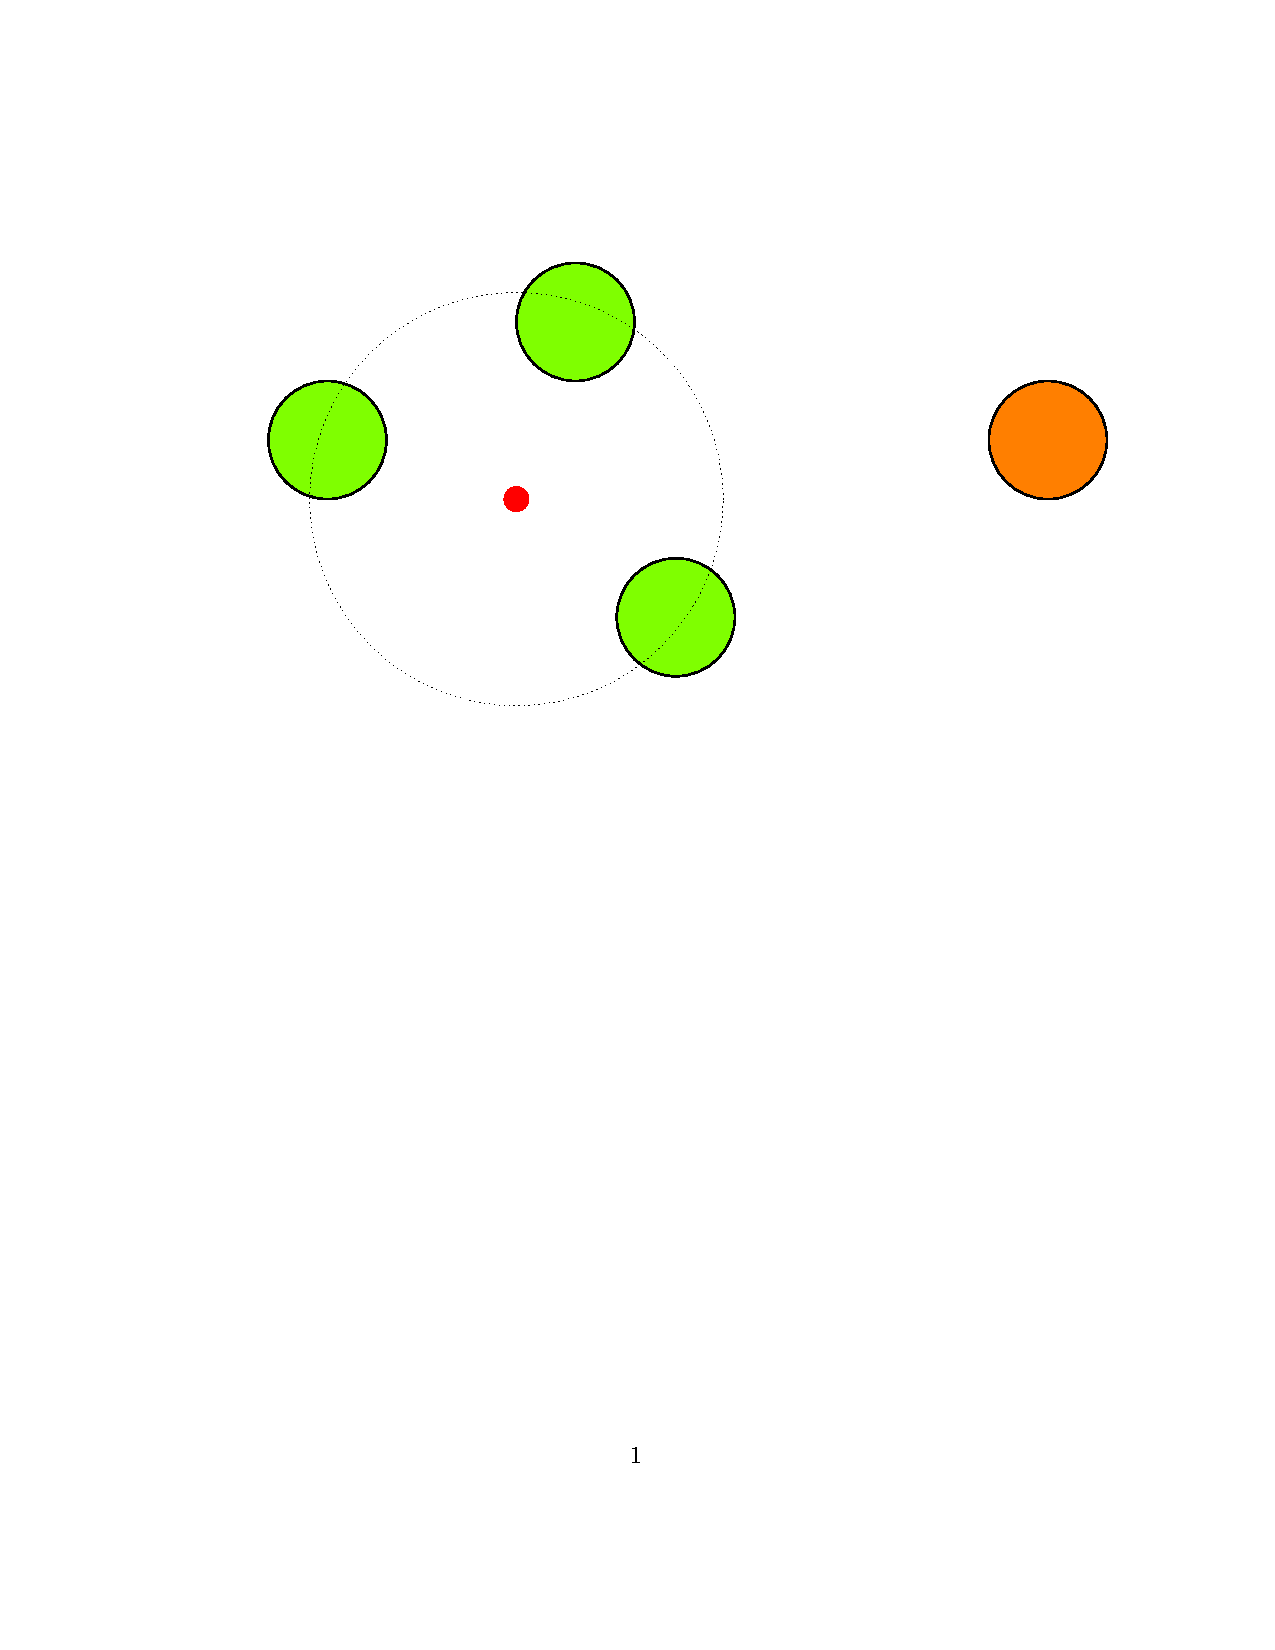
\includegraphics[trim = 100 0 0 100, clip, width=\linewidth]{figures/sparseDistanceSatisfied.pdf}
   \end{figure}
\end{frame}

\begin{frame}{Sparse-distance condition failure}   
   \begin{figure}
	  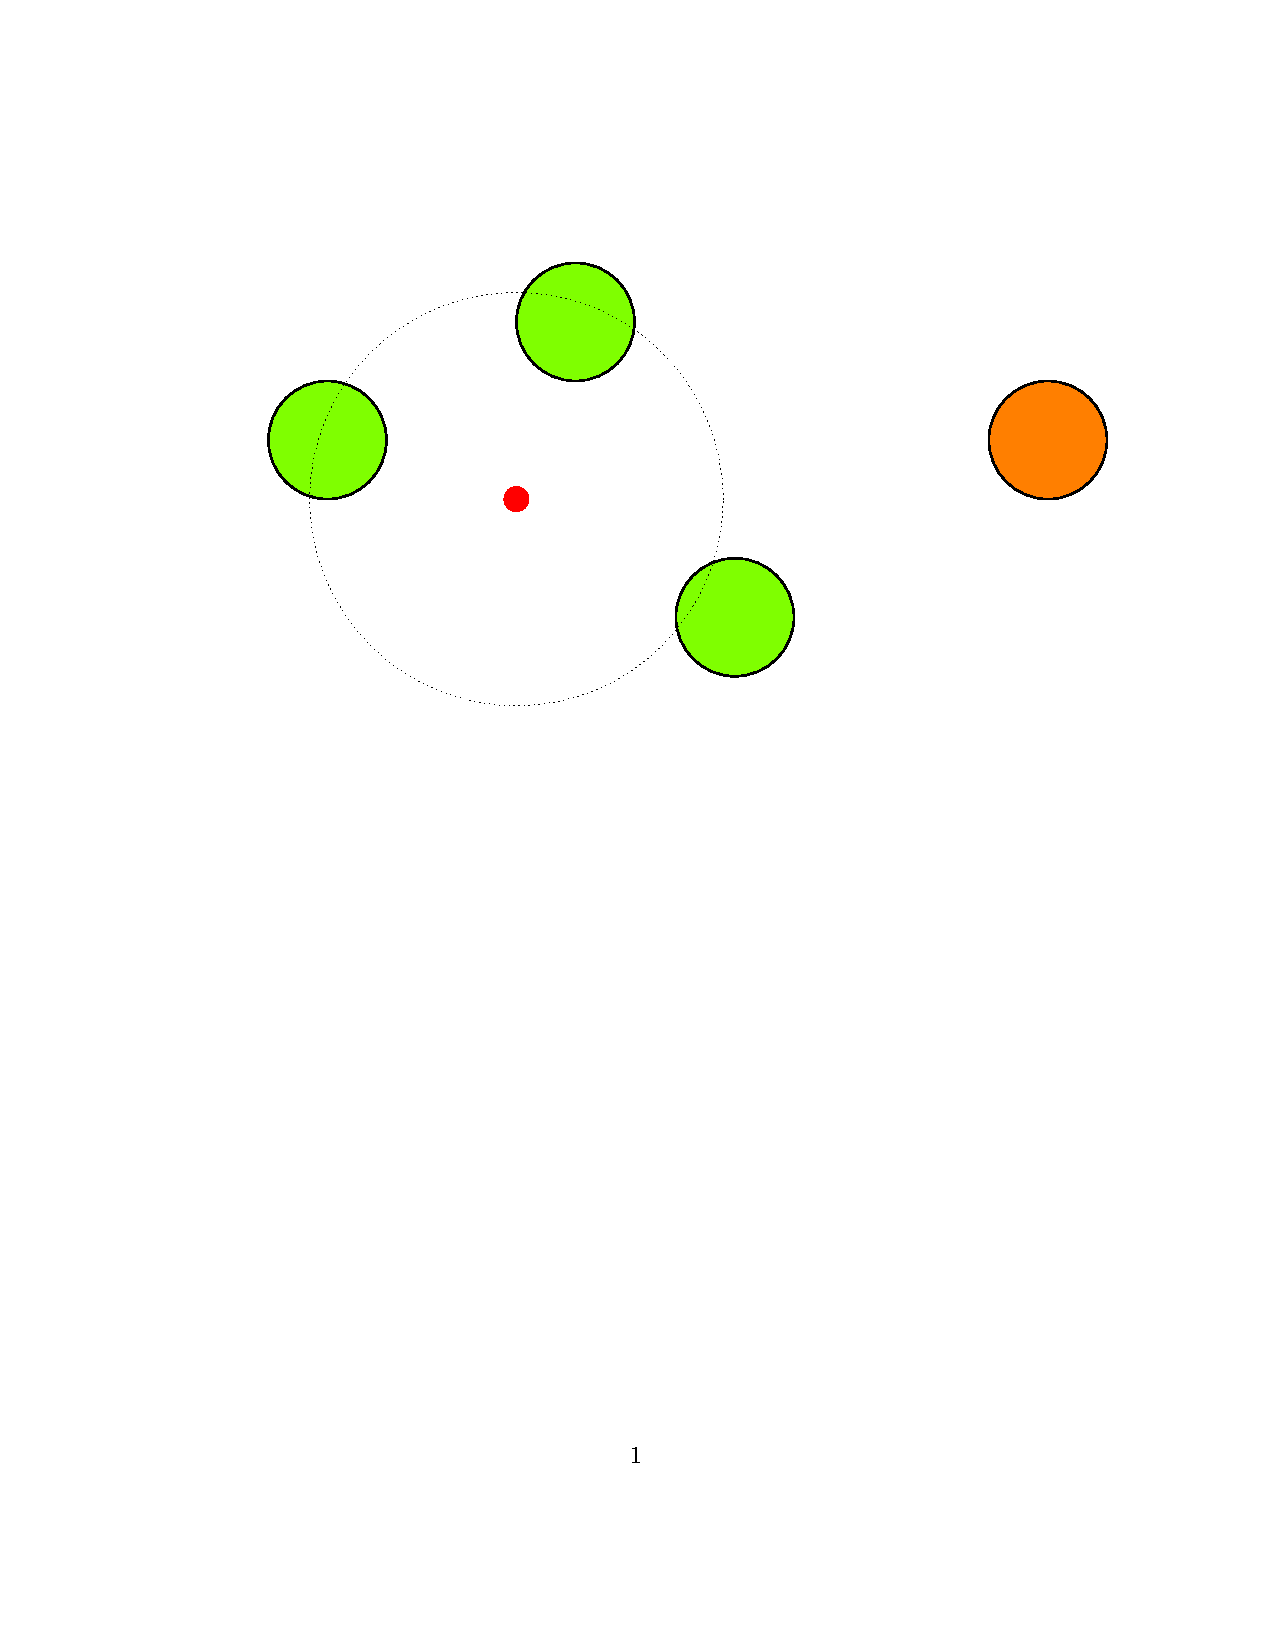
\includegraphics[trim = 100 0 0 100, clip, width=\linewidth]{figures/sparseDistanceNotSatisfied.pdf}
   \end{figure}
\end{frame}


\begin{frame}{Clustering under $(\alpha, \eta)$-center proximity}
	\begin{block}{The algorithm}
	  Input: $(\mc X, d)$ and a parameter $t$.\\
	  Output: A hierarchical clustering tree.\\
	  \vspace{0.1in}Initialize every point in its own cluster.\\
	  Go over all pairs of points $p, q$ in increasing order of distance.\\
	  If $B := B(p, d(p, q))$ satisfies the sparse-distance condition
	  \begin{itemize}
	  	\item Merge all clusters that intersect with $B$ into a single cluster
	  \end{itemize}
    \end{block}
\end{frame}

\begin{frame}{Lower bound}
	If $\alpha < 3 + \sqrt{2}$ and noise is sparse, then there doesn't exist a clustering tree which can capture all nice solutions.
	\begin{figure}[!t]
	  \begin{center}
	    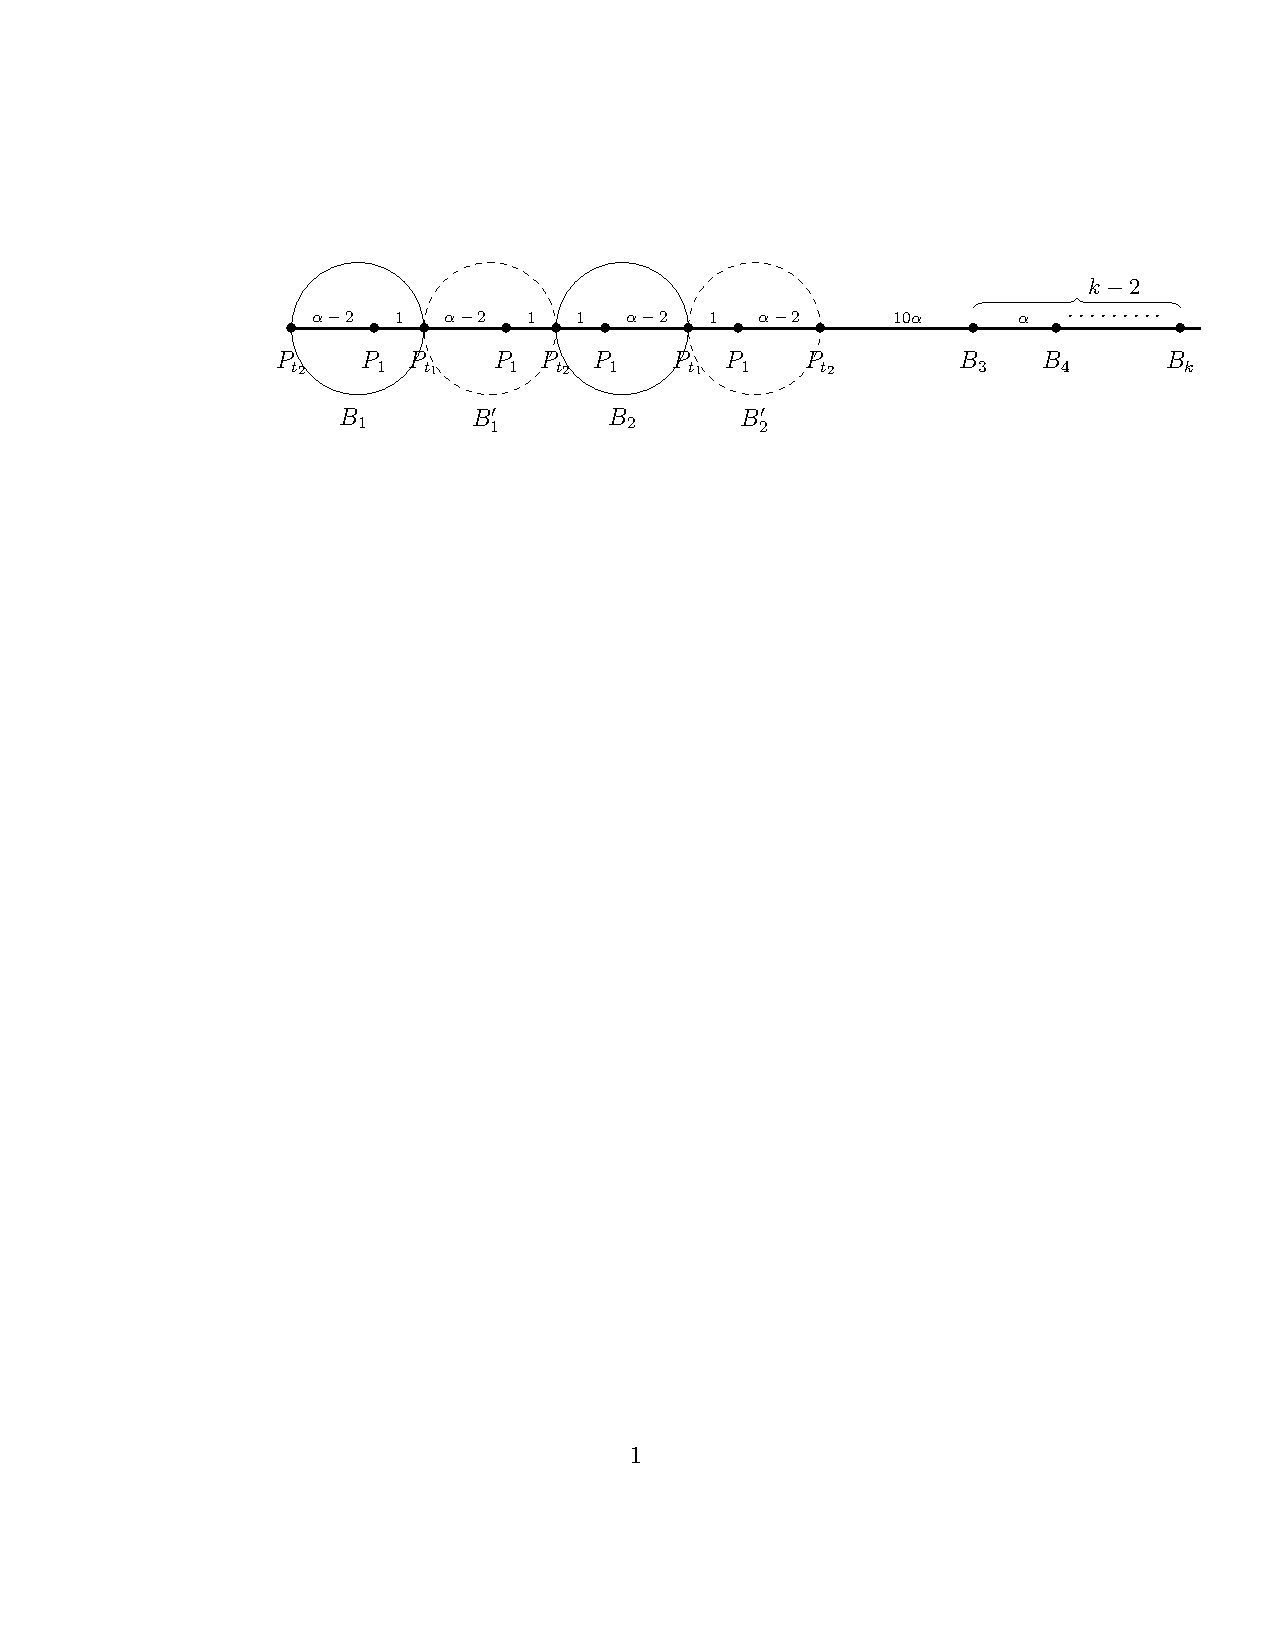
\includegraphics[trim={47mm 205mm 12mm 44mm},clip,width=\textwidth]{figures/lbdFig2.pdf}
	  \end{center}
	\end{figure}
	Same ideas can be extended to a list output. Any list should have size $> 2^{k/2}$
\end{frame}

\begin{frame}{Clustering is not easy}

  {\color{red}Challenges }
  \vspace{0.4cm}
  \vspace{0.3cm}\begin{itemize}
		\vspace{0.3cm}{\color{lb} \MyCitem  Computational Complexity }
		\vspace{0.3cm}\item Under-specificity
	\end{itemize}
\end{frame}

\begin{frame}{Under-specificity in clustering}
	
	Requirements from clustering algorithms\\
	\vspace{0.5cm}\begin{block}{}
	1. Similar points together\\
	\vspace{0.45cm}2. Dis-similar points separated
	\end{block}
	
	\vspace{0.5cm}These requirements can be conflicting
	\begin{center}
	\includegraphics[trim={100 650 30 120},clip,width=0.8\textwidth]{figures/conflictingReq.pdf}
	\end{center}
\end{frame}

\begin{frame}{Example}
	Given $\mc X \in \mb R^2$ and $k = 2$
	\begin{center}
	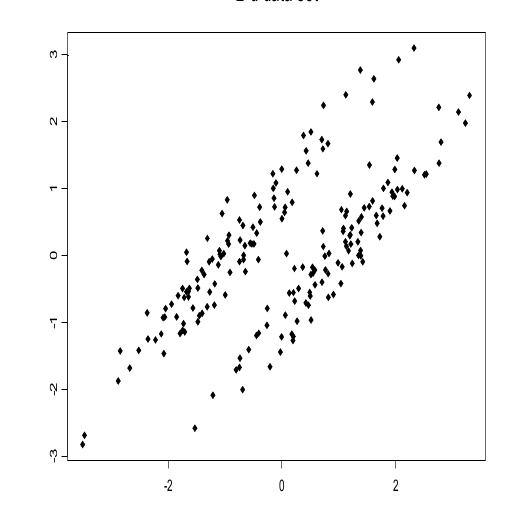
\includegraphics[trim={50 10 0 30},clip,width=0.5\textwidth]{figures/setX.png}
	\end{center}
\end{frame}

\begin{frame}{Example contd..}
	Given $\mc X \in \mb R^2$ and $k = 2$
	\begin{center}
	\begin{figure}
	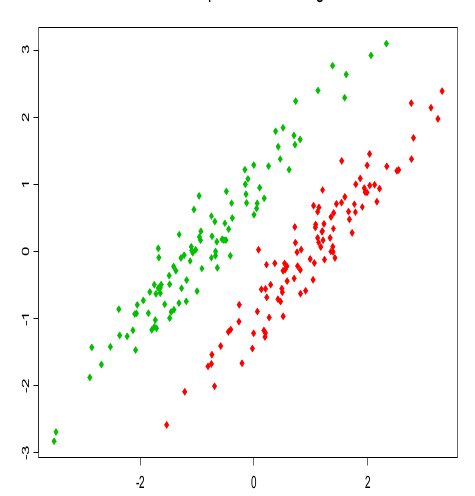
\includegraphics[trim={0 0 0 20},clip,width=0.4\textwidth]{figures/slX.png}
	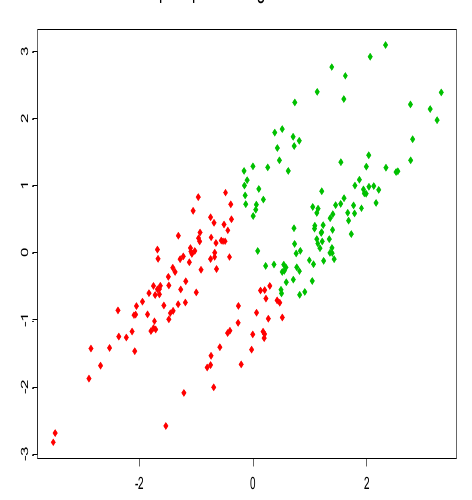
\includegraphics[trim={0 0 0 20},clip,width=0.4\textwidth]{figures/kmeansX.png}
	\caption{Single-linkage on our example dataset (Left). $K$-means on our example dataset (Right)}
	\end{figure}
	\end{center}
\end{frame}

\begin{frame}{Considerations of different algorithms}
	
	{\color{blue}Single-linkage}\\
	\vspace{0.3cm}Tries to put \alert{similar} points together\\
	\vspace{0.3cm}Can end-up having dissimilar points together.\\
	
	\vspace{1cm}{\color{blue}$K$-Means}\\
	\vspace{0.3cm}Tries to \alert{separate} dissimilar points\\
	\vspace{0.3cm}Can end-up separating similar points.\\
	
\end{frame}

\begin{frame}{The problem of under-specificity}
	Different application require different approaches\\
	\vspace{1cm} How to prefer one choice over the other?\\
	\vspace{1.5cm} Add {\color{blue} bias} to express {\color{blue} prior domain knowledge}
\end{frame}

\begin{frame}{Previous approach to tackle under-specificity}
	
	{\color{blue}Must/cannot} link constraints \alert{[Basu et. al `02]}\\
	\vspace{1cm}Sub-sample clustering \alert{[Ashtiani, Ben-David `15]}\\
	\vspace{1cm}{\color{blue}Merge/split} queries \alert{[Balcan, Blum `08]}
\end{frame}

\begin{frame}{Our approach to tackle under-specificity}
	
	{\color{blue}Same-cluster query}\\
    \vspace{1cm}Given a clustering $\mc C$ of set $\mc X$\\
    \vspace{0.51cm}Ask same-cluster queries to a ${\mc C}$-oracle\\
    $$f_{\mc C}(x_1, x_2) = \left\{
	\begin{array}{ll}
		\mbox{true }  & \mbox{if } x_1 \overset{\mc C}{\sim} x_2   \\
		\mbox{false } & otherwise 
	\end{array}
\right. $$
\end{frame}

\begin{frame}{Problem Setting}
	Input: $(\mc X, d)$
	\begin{itemize} 
   		\vspace{0.4cm}\item Learner can make same-cluster queries to $\mc C$-oracle
		\vspace{0.4cm}\item Oracle's clustering is ``nice".     
	\end{itemize}
	\vspace{1.4cm} Recover the oracle's clustering $\mc C=(C_1, \ldots, C_k)$
\end{frame}

\begin{frame}{$\gamma$-margin niceness}
	Cluster-center is closer to its own points than to points outside.\\
	\vspace{1cm}$\gamma$ controls the separation.
	\vspace{1cm}\begin{figure}        
            \centering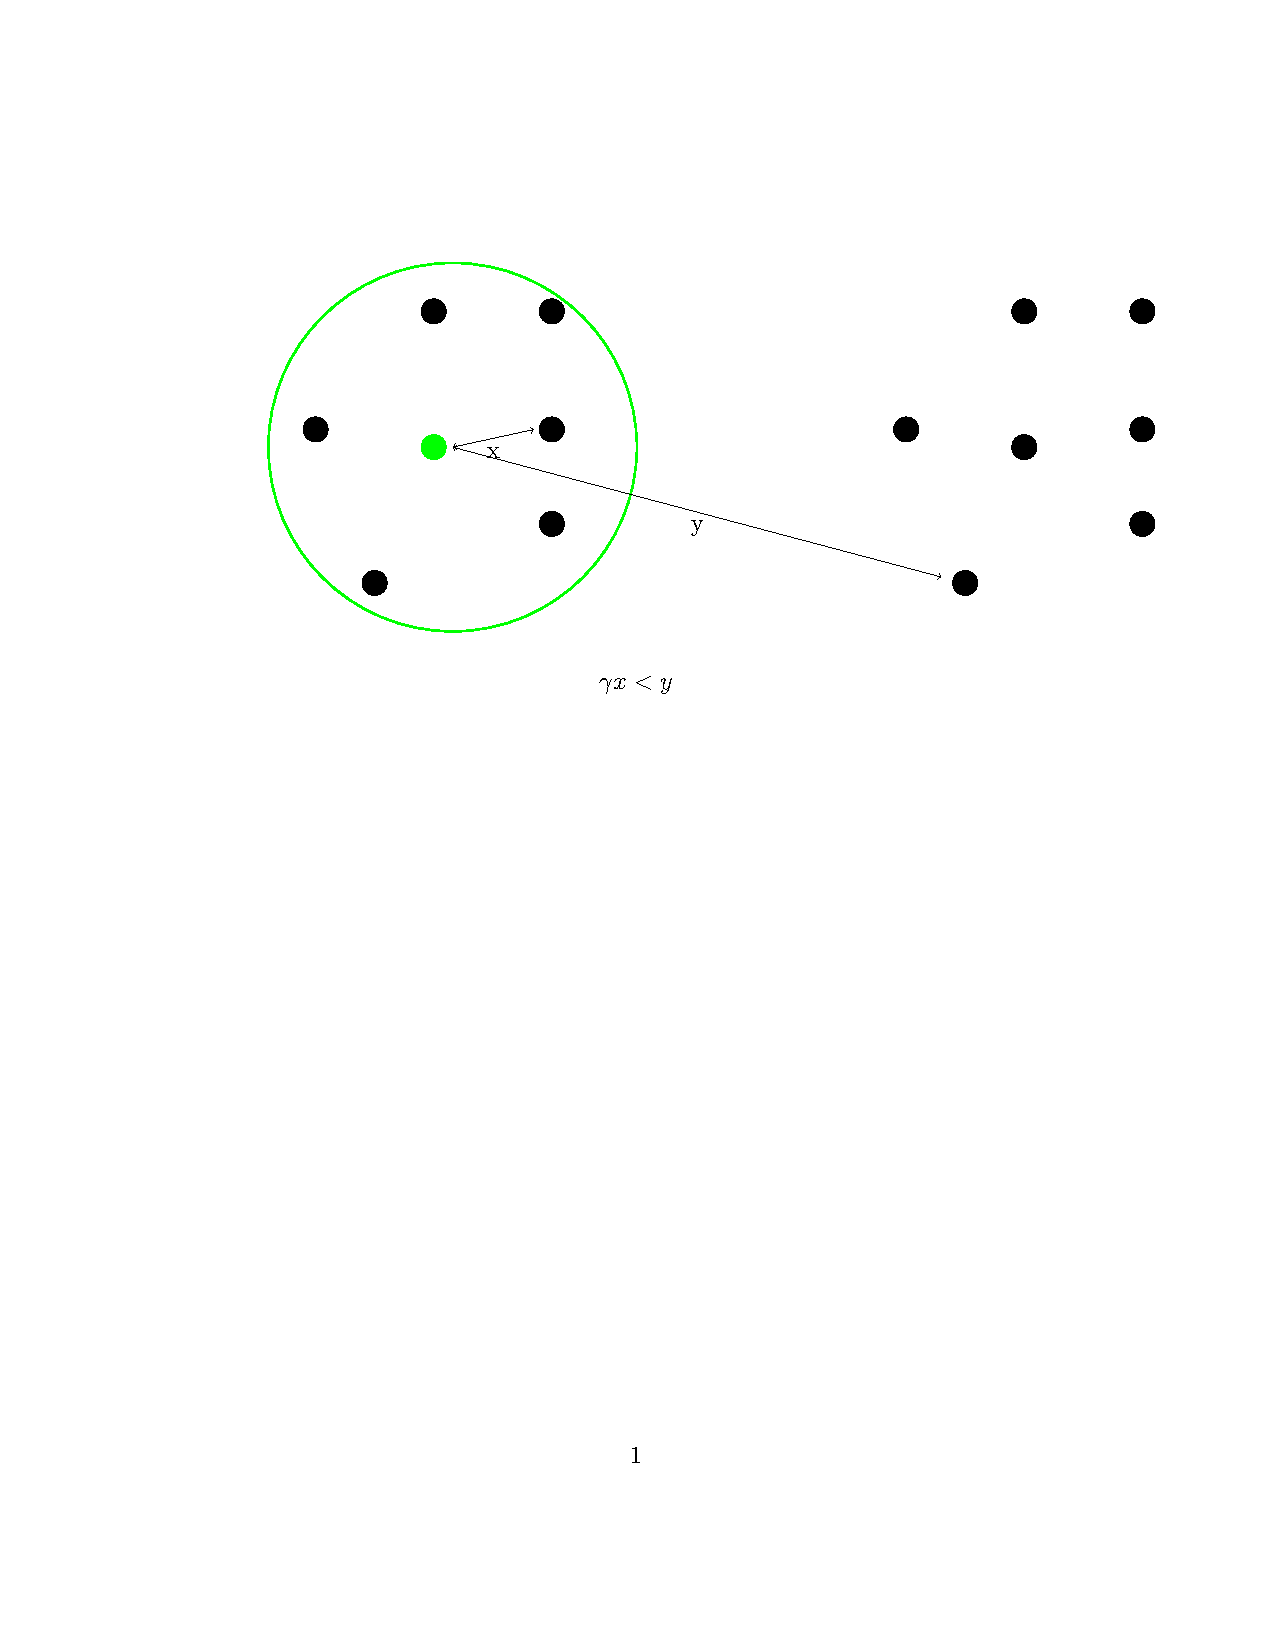
\includegraphics[trim= 400 470 400 150, scale=0.5]{figures/gammaMargin.pdf}
    \end{figure}  
\end{frame}

\begin{frame}{Formally $\ldots$}
	Given $(\mc X, d)$ and $k$.\\
	\vspace{0.4cm}Clustering $\mc C$ induced by centers $\mu_1, \ldots, \mu_k$\\
	
	\vspace{1cm}\begin{block}{}
		For all $i$, for all $x \in C_i$ and for all $y \not\in C_i$
		$$\gamma d(x, \mu_i) < d(y, \mu_i)$$	
	\end{block}  
\end{frame}

\begin{frame}{Margin vs center-proximity (no queries)}
  Given $(\mc X, d)$ and $k$\\
  \vspace{0.5cm}Optimal $k$-means solution satisifies nice property ($\gamma$-margin or $\alpha$-center proximity)

	\begin{table}[]
	\centering
	%\caption{My caption}
	\label{my-label}
	\begin{tabular}{llllll}
	\multicolumn{1}{c}{} &  &  & \begin{tabular}[c]{@{}l@{}}$\alpha$-center \\ proximity\end{tabular} &  & \begin{tabular}[c]{@{}l@{}}$\gamma$-margin\end{tabular} \\
	 &  &  &  &  &  \\
	K-means &  &  & \begin{tabular}[c]{@{}l@{}}upper bound: 3.7\\ lower bound: 3\end{tabular} &  & \begin{tabular}[c]{@{}l@{}}upper bound: 3\\ lower bound: 3\end{tabular} \\
	K-median &  &  & \begin{tabular}[c]{@{}l@{}}upper bound: 2.4\\ lower bound: 2\end{tabular} &  & \begin{tabular}[c]{@{}l@{}}upper bound: 2\\ lower bound: 2\end{tabular}
	\end{tabular}
	\end{table}
\end{frame}

\begin{frame}{Problem Setting}
	Input: $(\mc X, d)$
	\begin{itemize} 
   		\vspace{0.4cm}\item Learner can make same-cluster queries to $\mc C$-oracle
		\vspace{0.4cm}\item Oracle's clustering satisfies $\gamma$-margin     
	\end{itemize}
	\vspace{1.4cm} Recover the oracle's clustering $\mc C=(C_1, \ldots, C_k)$
\end{frame}

\begin{frame}{Our Results}
  \alert{Positive result}
  \vspace{0.5cm}
  \begin{itemize}
    
    \item $\gamma > 1$ \\
    \vspace{0.3cm} \textcolor{blue}{Our algorithm finds the} \textcolor{red}{target} \textcolor{blue}{clustering with high probability}
    
    \begin{itemize}
    	\vspace{0.3cm}
        \item Runs in $O(kn\log n)$
        \vspace{0.3cm}
        \item Asks $O(k^2\log k + k\log n)$ queries
    \end{itemize}
   \end{itemize}
\end{frame}

\begin{frame}{$K$-means revisited}
	Input: $\mc X \subseteq \mb R^d$ and $k$\\
	\vspace{0.5cm}Find $\mu_1, \ldots, \mu_k$ so as to minimize
	$$\sum_{i=1}^k \sum_{x \in C_i} \|x - \mu_i\|^2$$
	
	\vspace{1cm}\alert{Additional information}\\
	\vspace{0.5cm} The optimal solution satisfies $\gamma$-margin.
\end{frame}

\begin{frame}{$K$-means revisted}
	\alert{Negative result without queries} 
	\vspace{0.5cm}
    \begin{itemize}
	    \item $\gamma < 1.84$ \\
	    \vspace{0.3cm} {NP-Hard to find an optimal}
	\end{itemize}

	\vspace{1cm}\color{blue}{Positive result with queries} 
	\vspace{0.5cm}
    \begin{itemize}
	    \item $\gamma > 1$ \\
	    \vspace{0.3cm} {Efficiently find the optimal using $O(\log n)$ queries}
	\end{itemize}
\end{frame}

\begin{frame}{Surprising Conclusion}

    \begin{block}{}
    \begin{center}{\Large NP-hard for $\gamma<1.84$\\
      \vspace{0.2cm}\textbf{BUT} \\
      \vspace{0.3cm}tractable with $O(\log n)$ queries.}
    \end{center}
    \end{block}
\end{frame}

\begin{frame}{Clustering with Queries}
  \begin{block}{The algorithm}
	\vspace{0.2cm}Input: $(\mc X, d)$, $k$ and parameters $\gamma$ and $\delta$.\\
    \vspace{0.2cm}Output: A clustering of $\mc X$.\\
	\vspace{0.4cm}
	1. Estimate center\\
	\begin{itemize}
		\item Query uniformly till we have ``enough'' points from one cluster
    \end{itemize}  
	\vspace{0.4cm}
	2. Compute radius\\
	\begin{itemize}
	  \vspace{0.2cm}
	  \item Binary search to find the ``radius"
    \end{itemize}  
	\vspace{0.4cm}
	3. Delete and repeat
  \end{block}
\end{frame}

\begin{frame}{Algorithm}
	\only<1>{\centering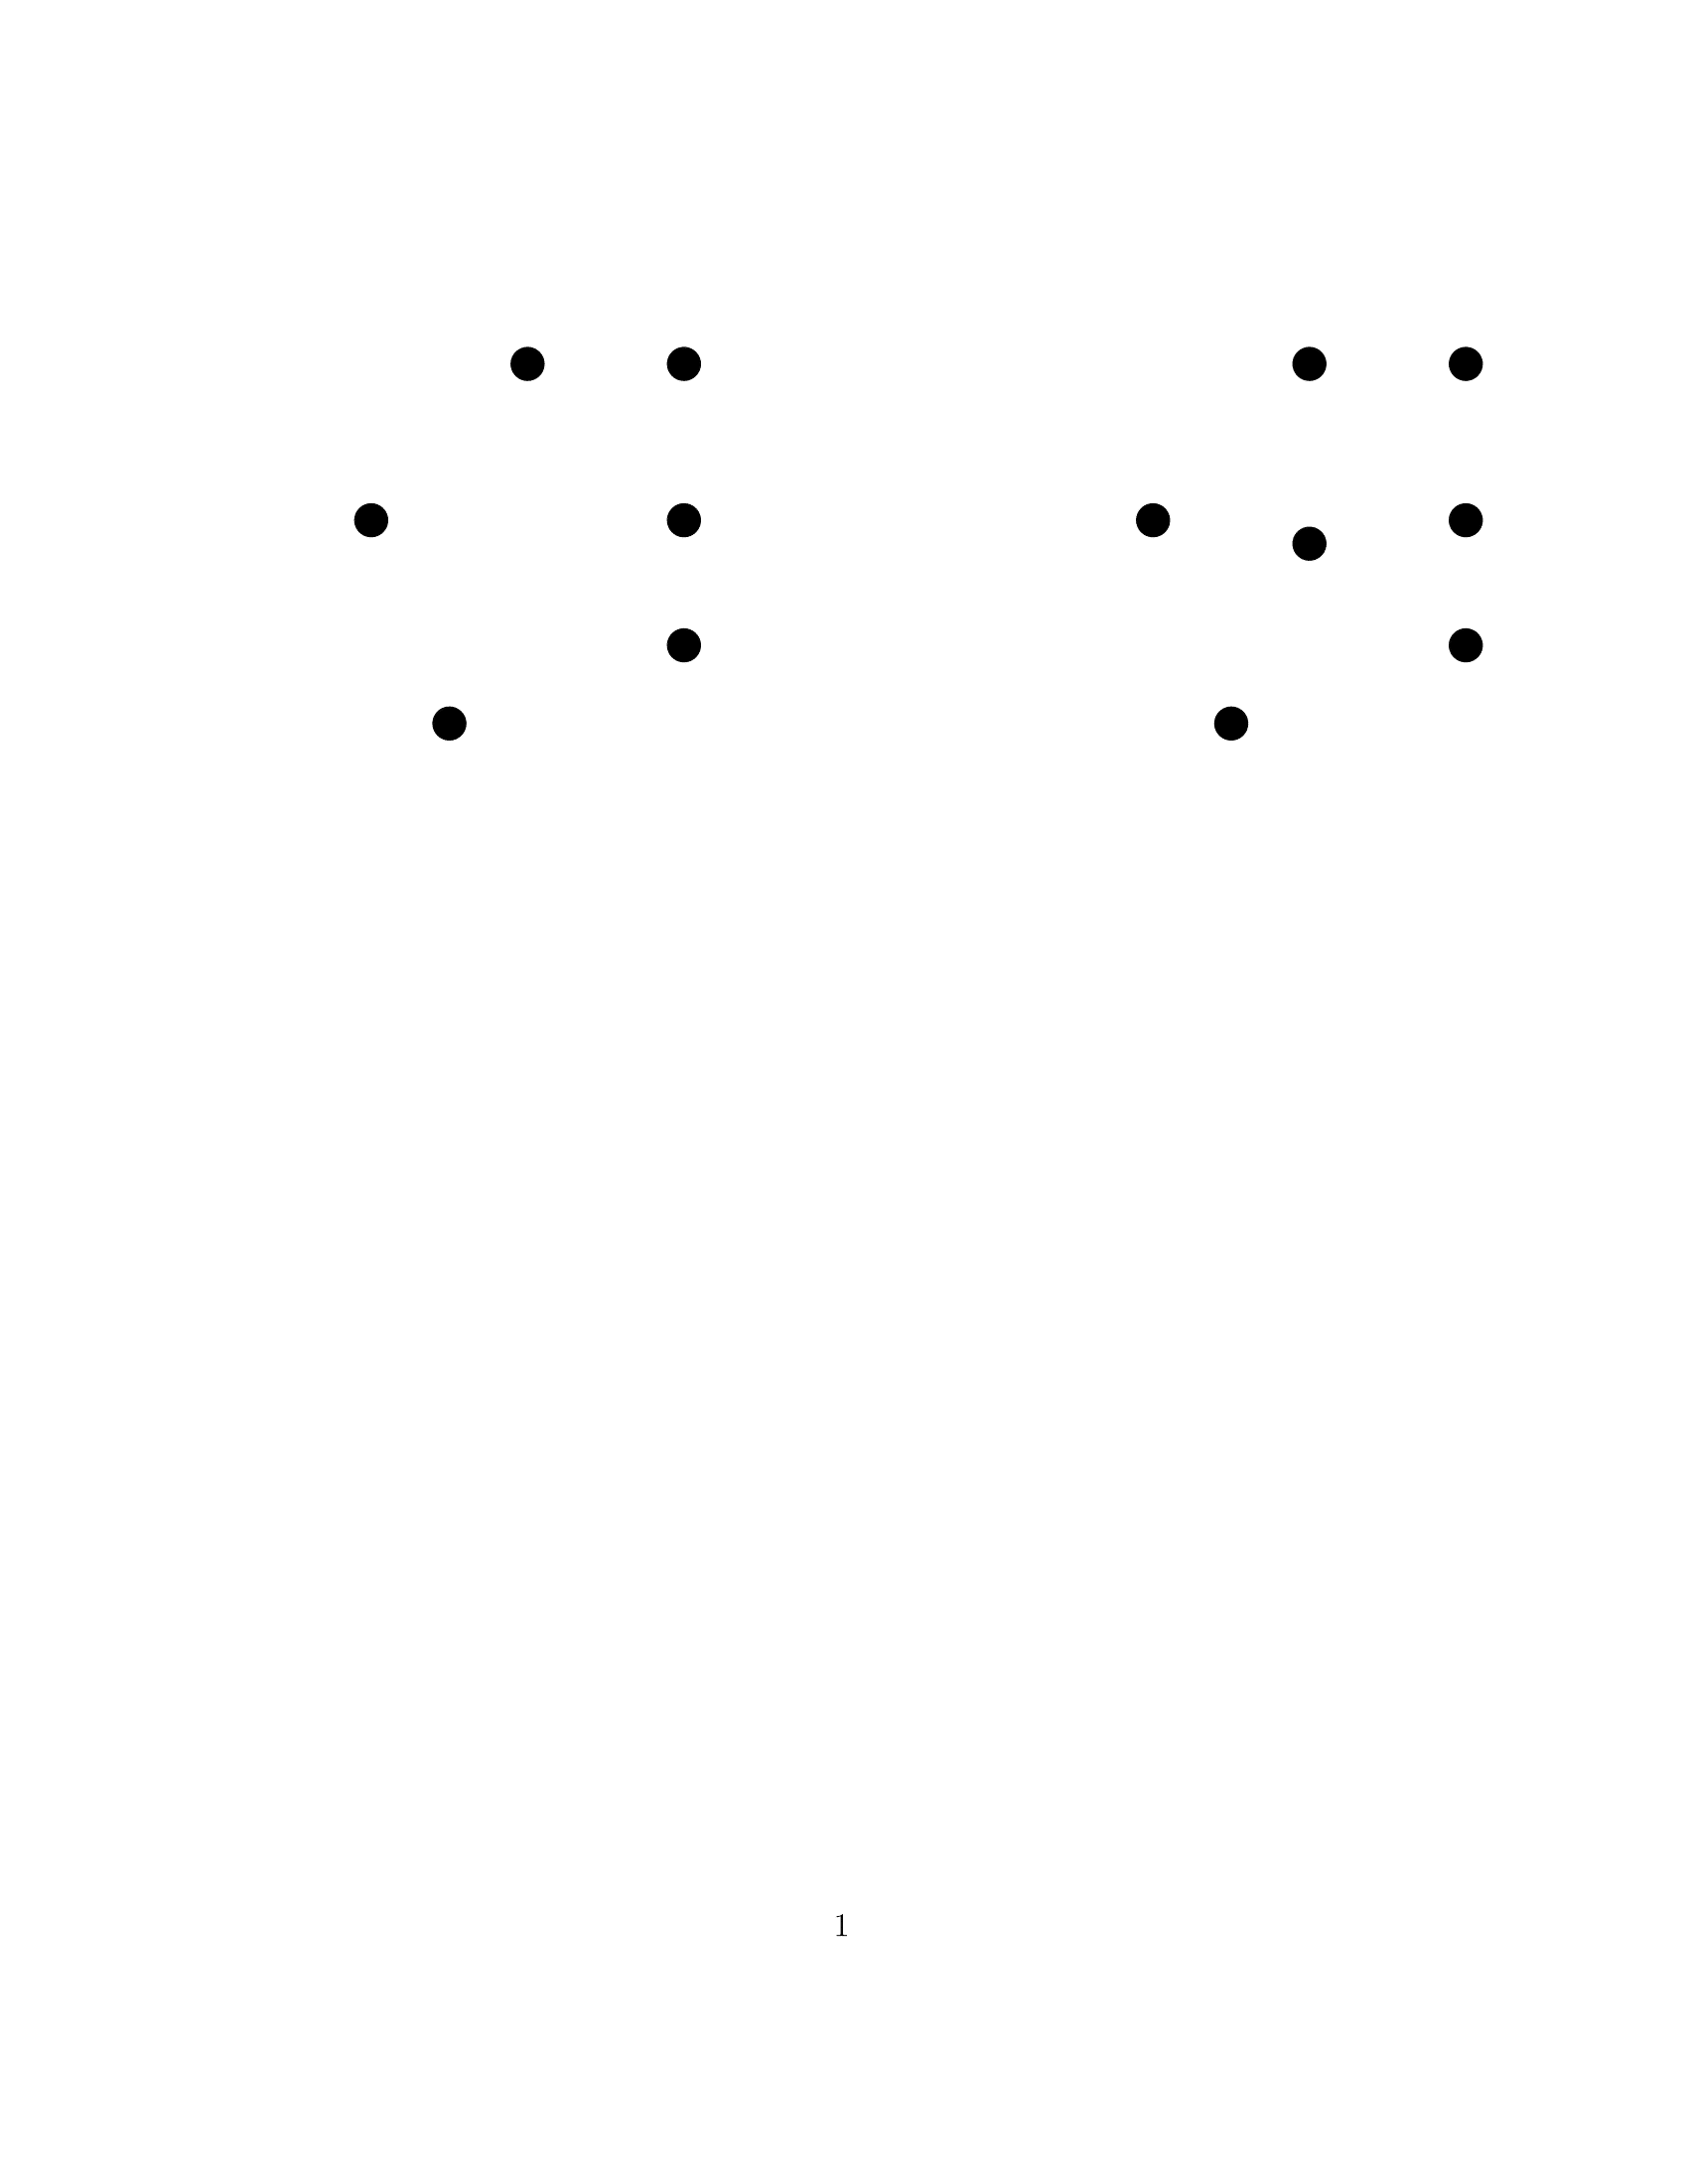
\includegraphics[scale=0.15]{figures/gammaAlg/gammaAlgo-0.png}}
	\only<2>{\centering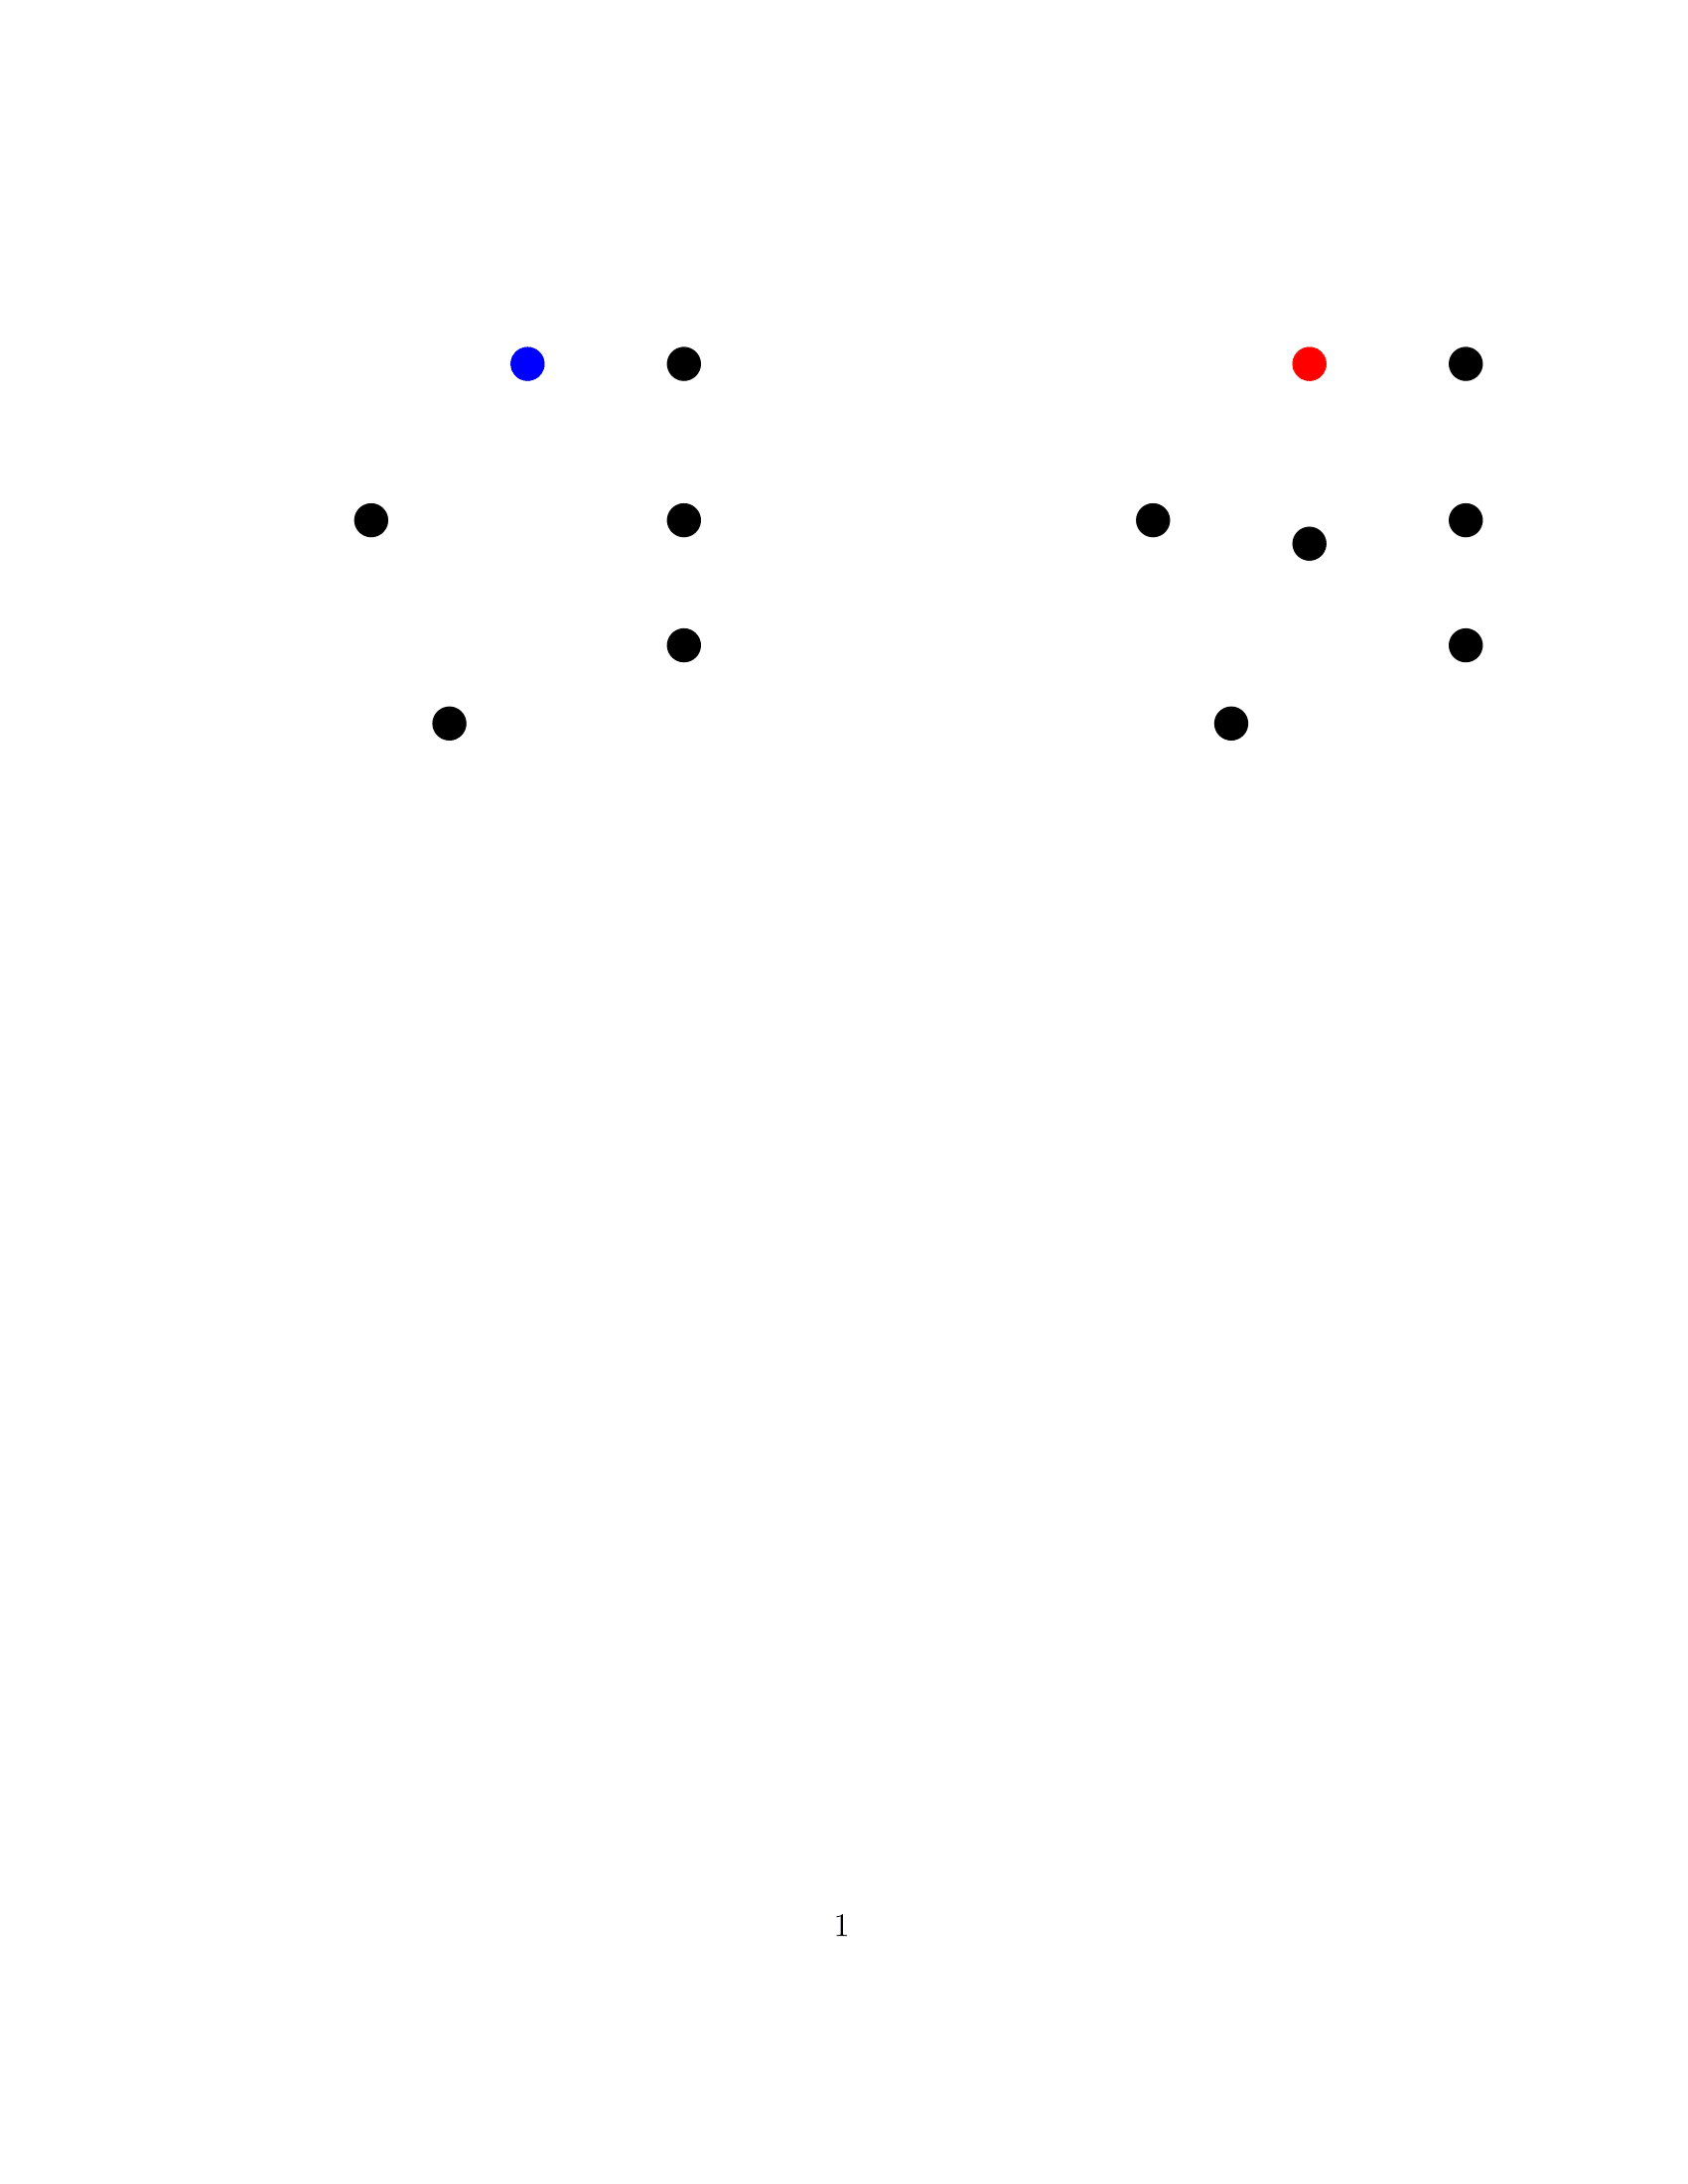
\includegraphics[scale=0.15]{figures/gammaAlg/gammaAlgo-1.png}}
	\only<3>{\centering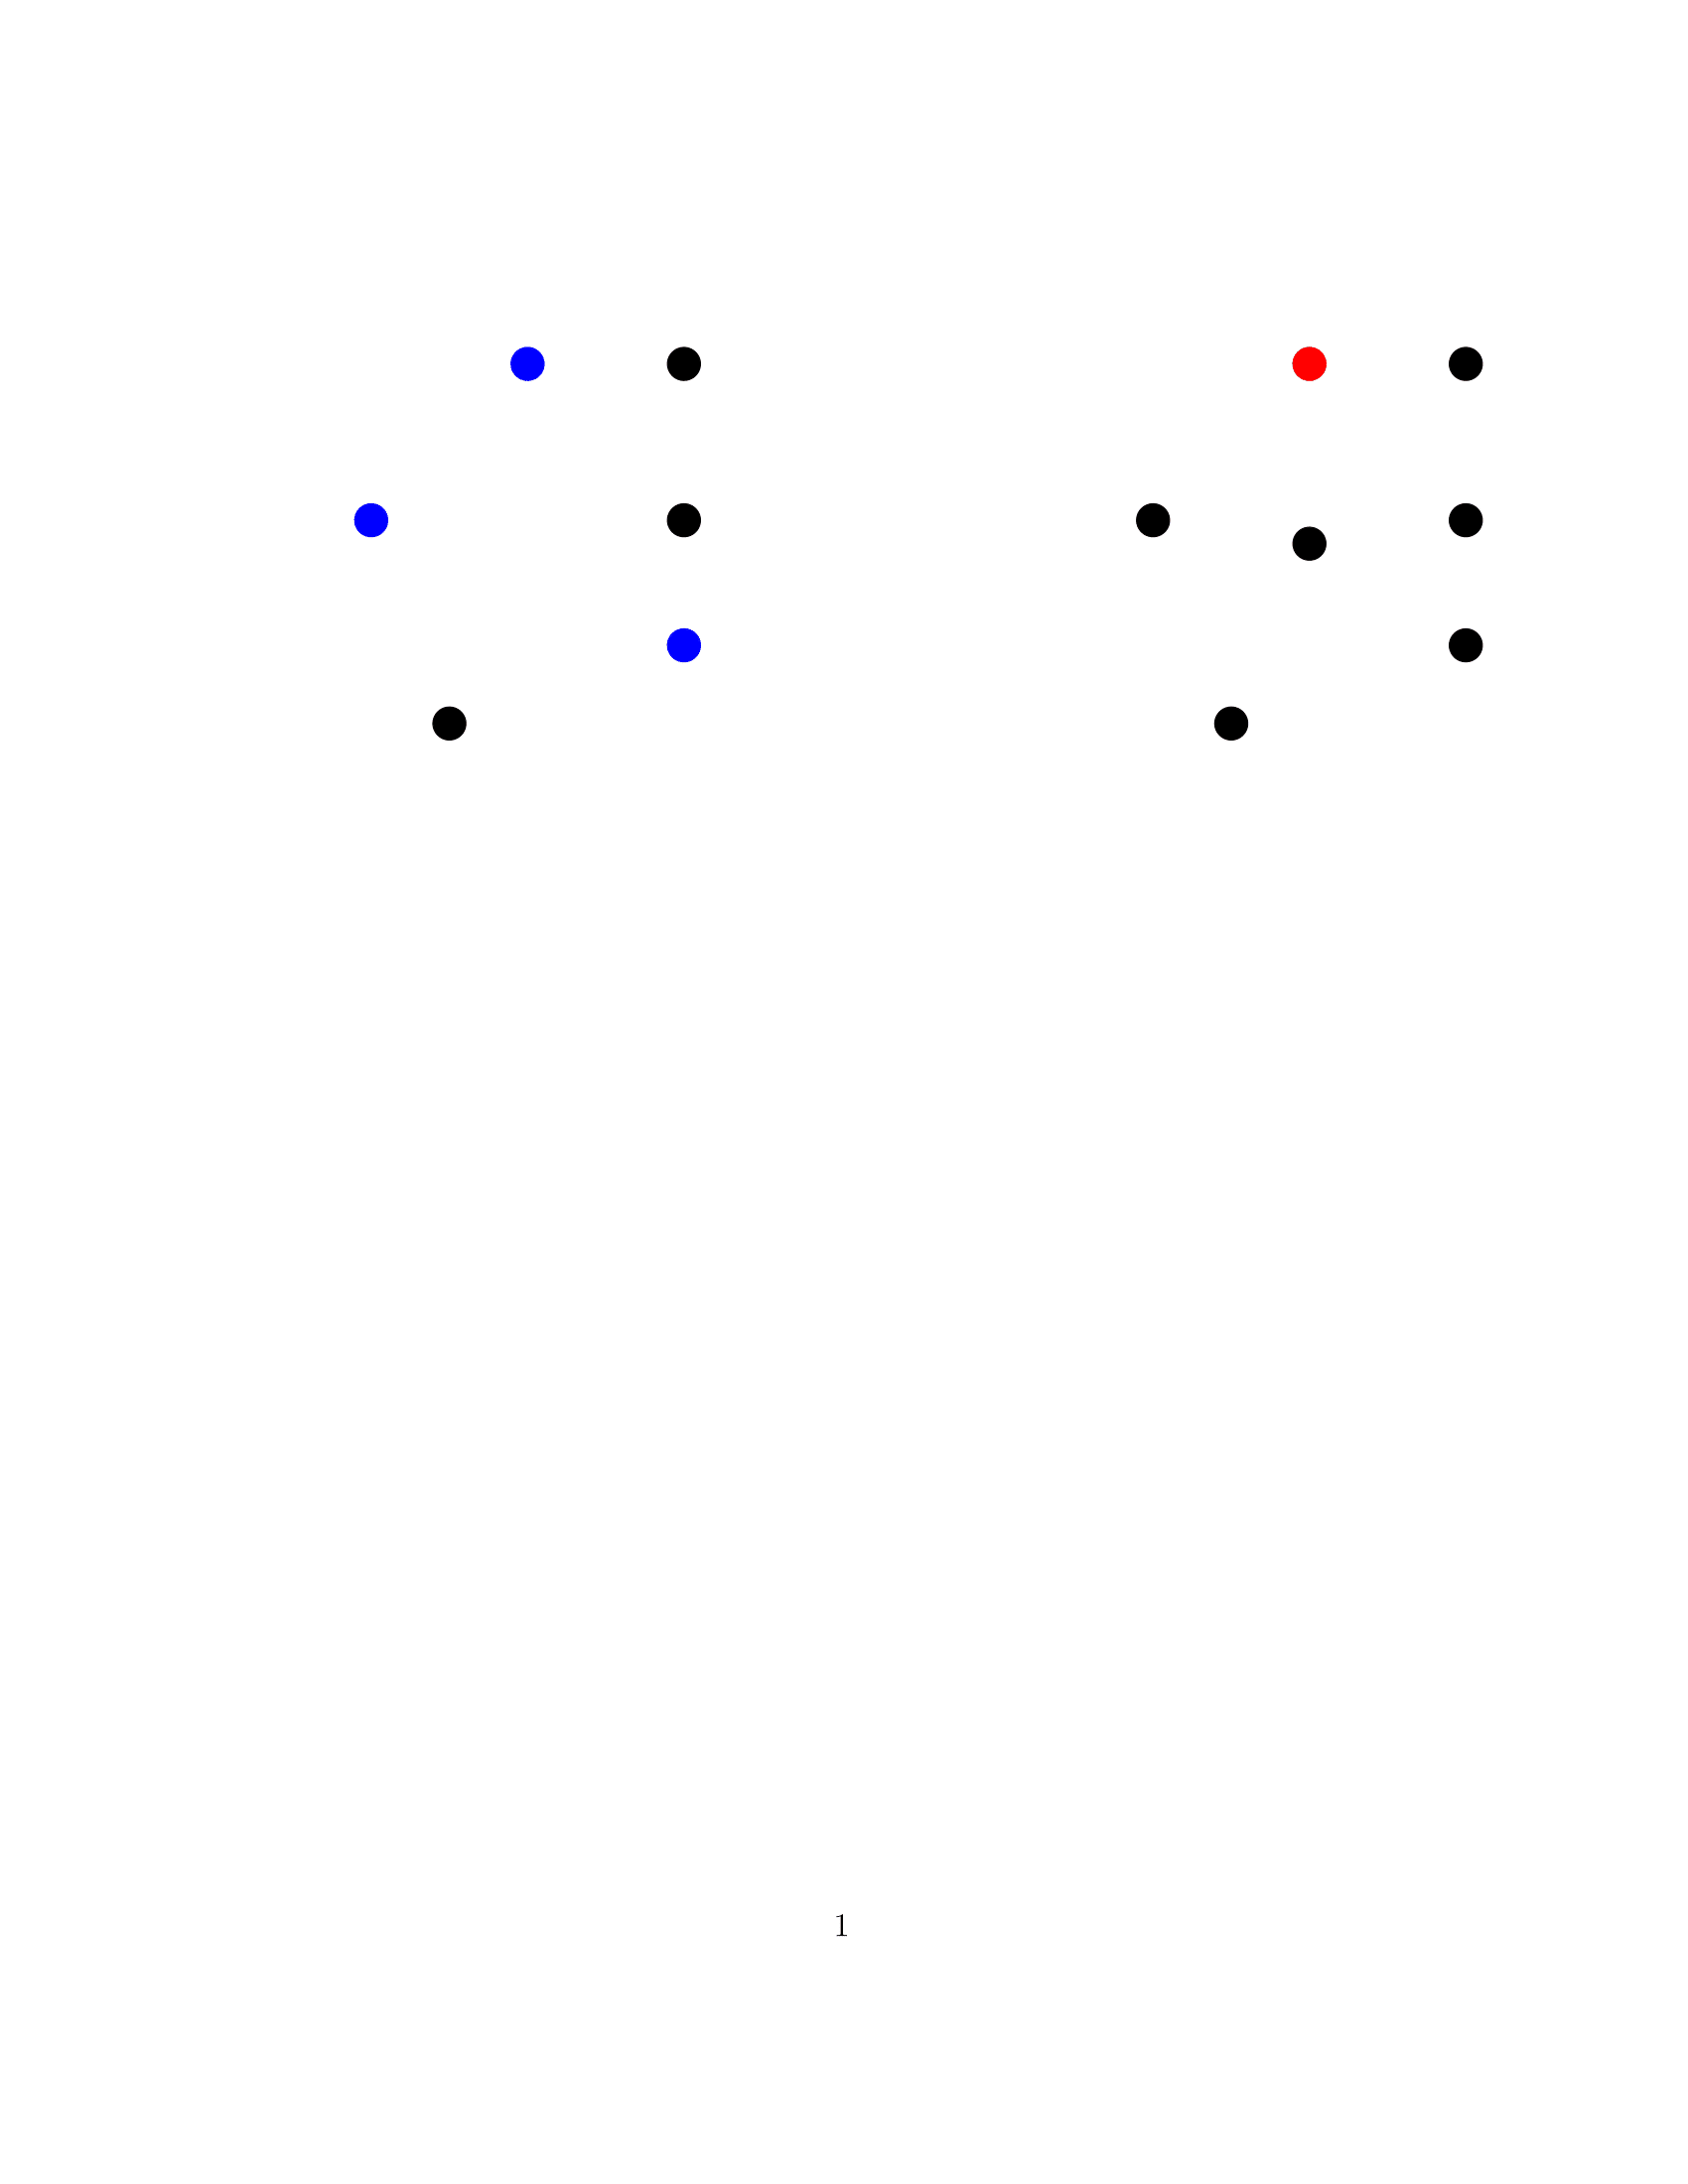
\includegraphics[scale=0.15]{figures/gammaAlg/gammaAlgo-2.png}}
	\only<4>{\centering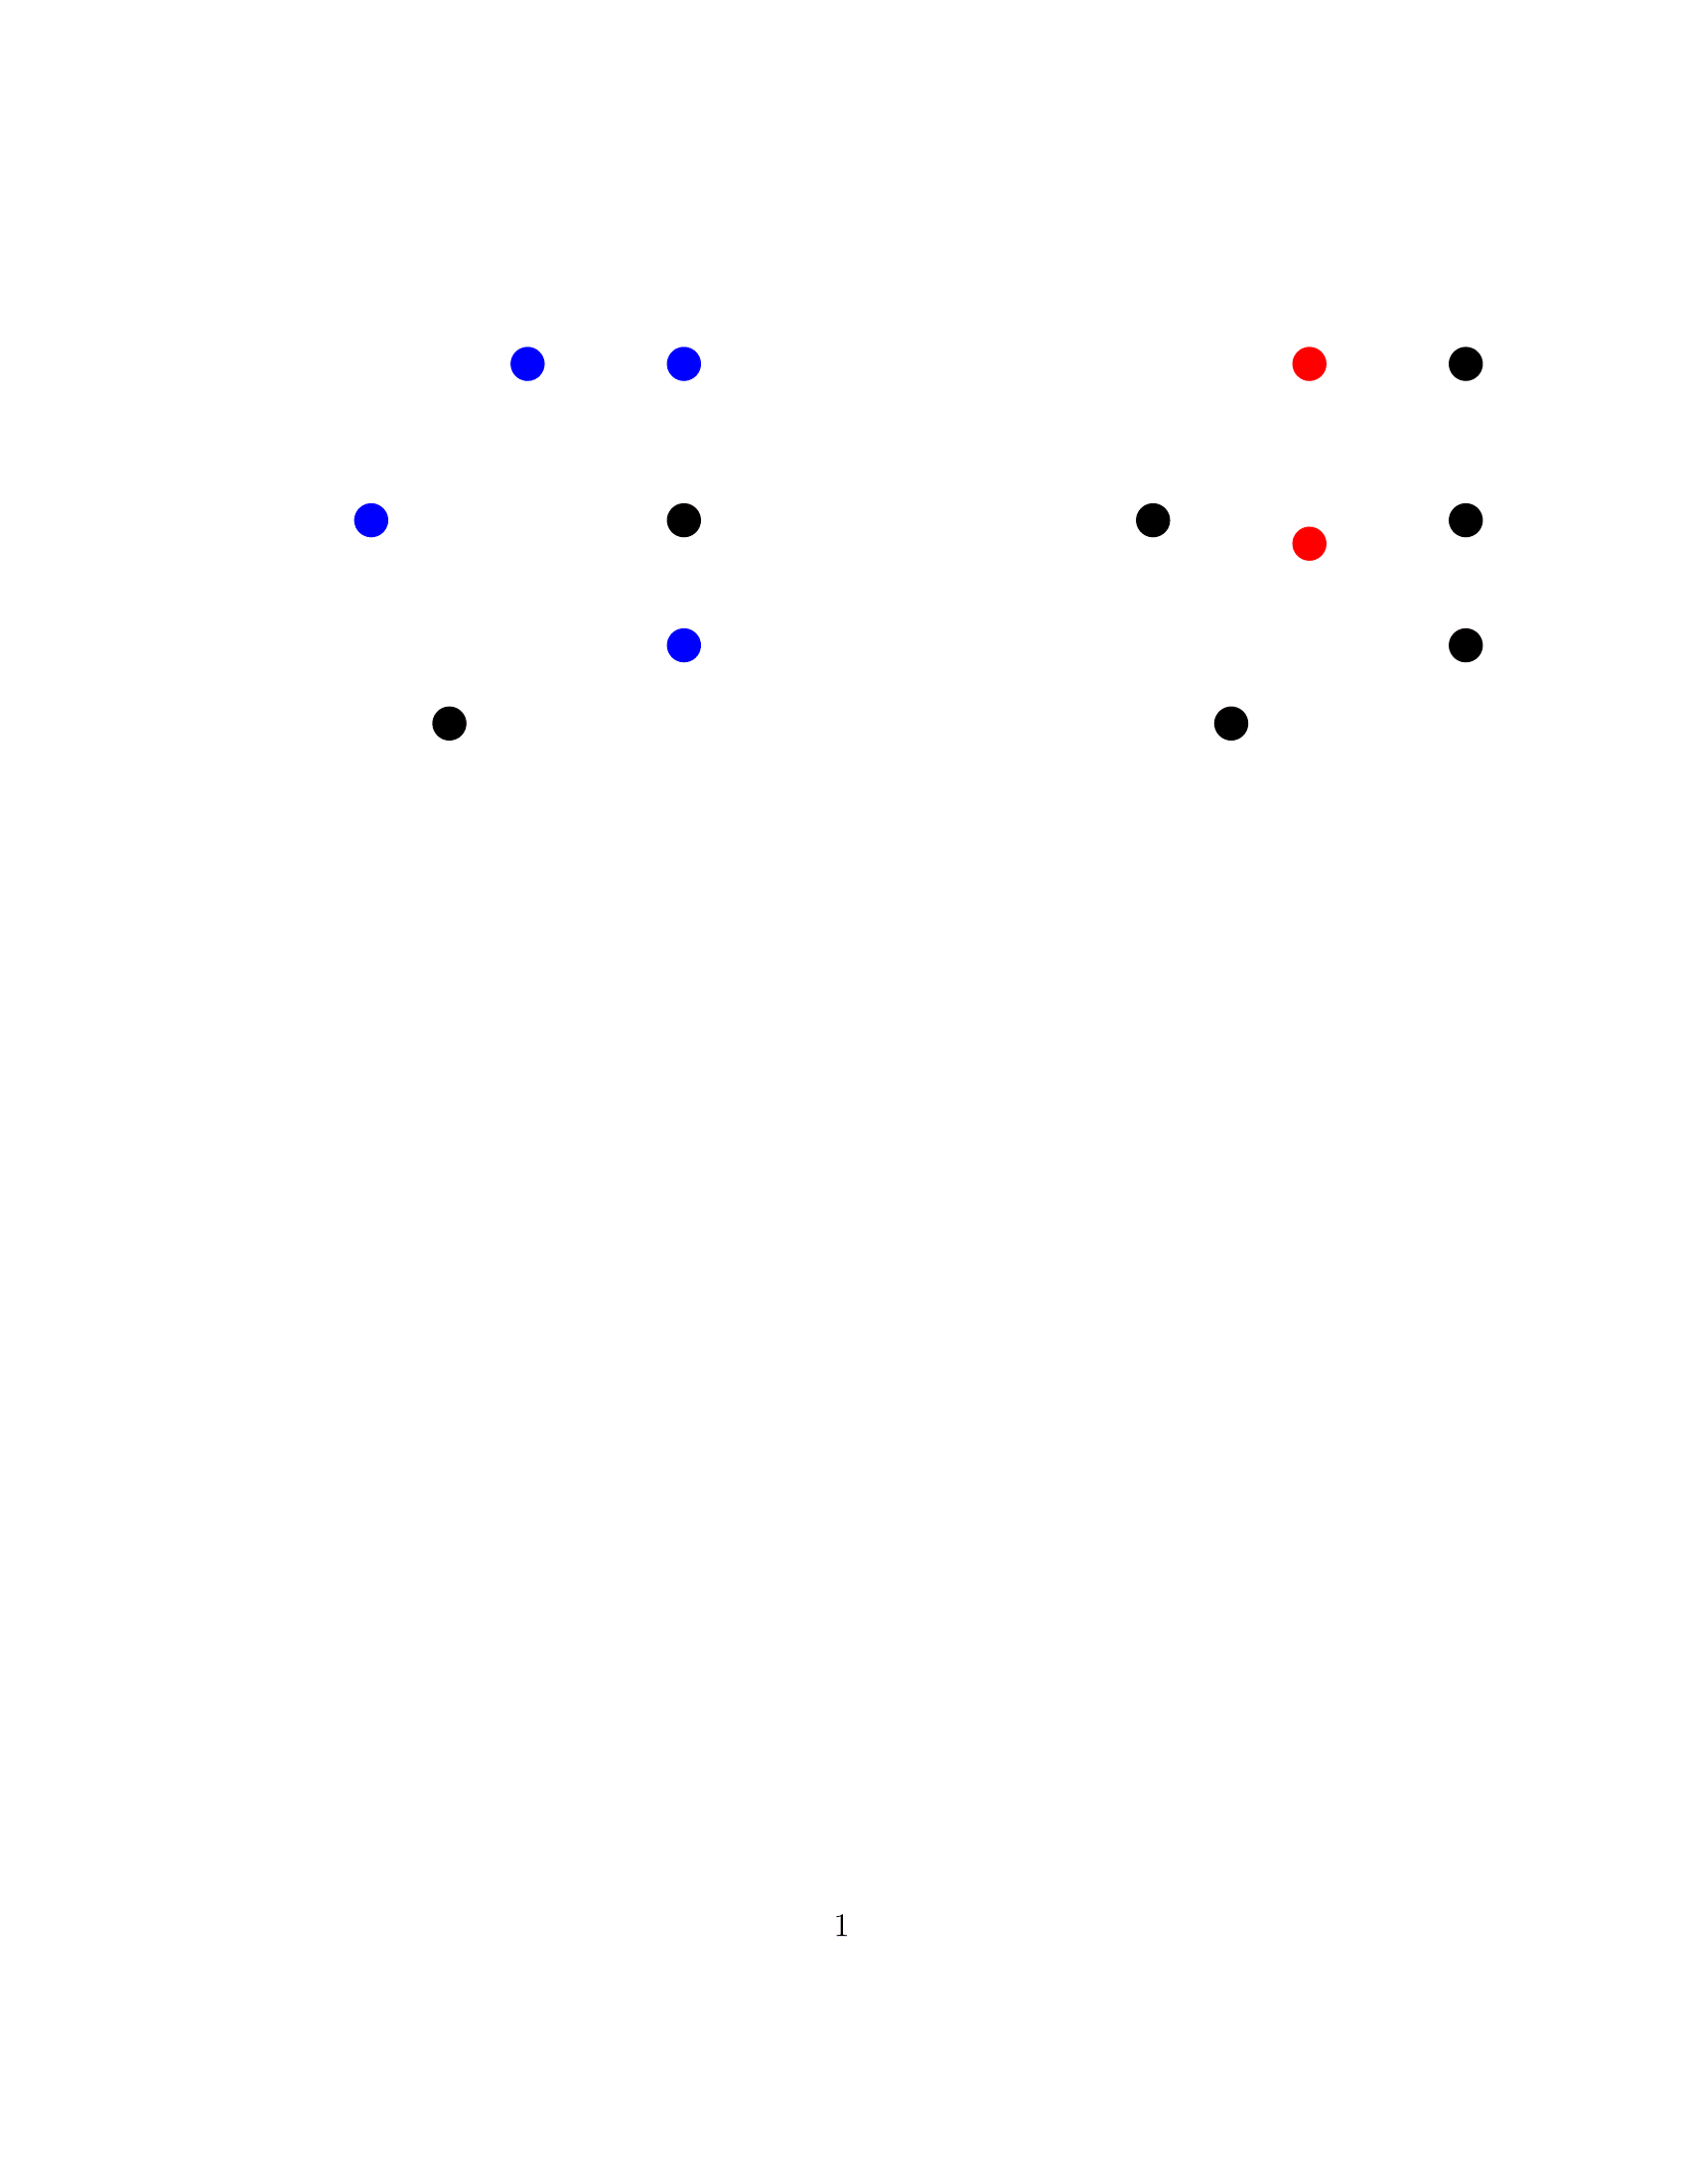
\includegraphics[scale=0.15]{figures/gammaAlg/gammaAlgo-3.png}}
	\only<5>{\centering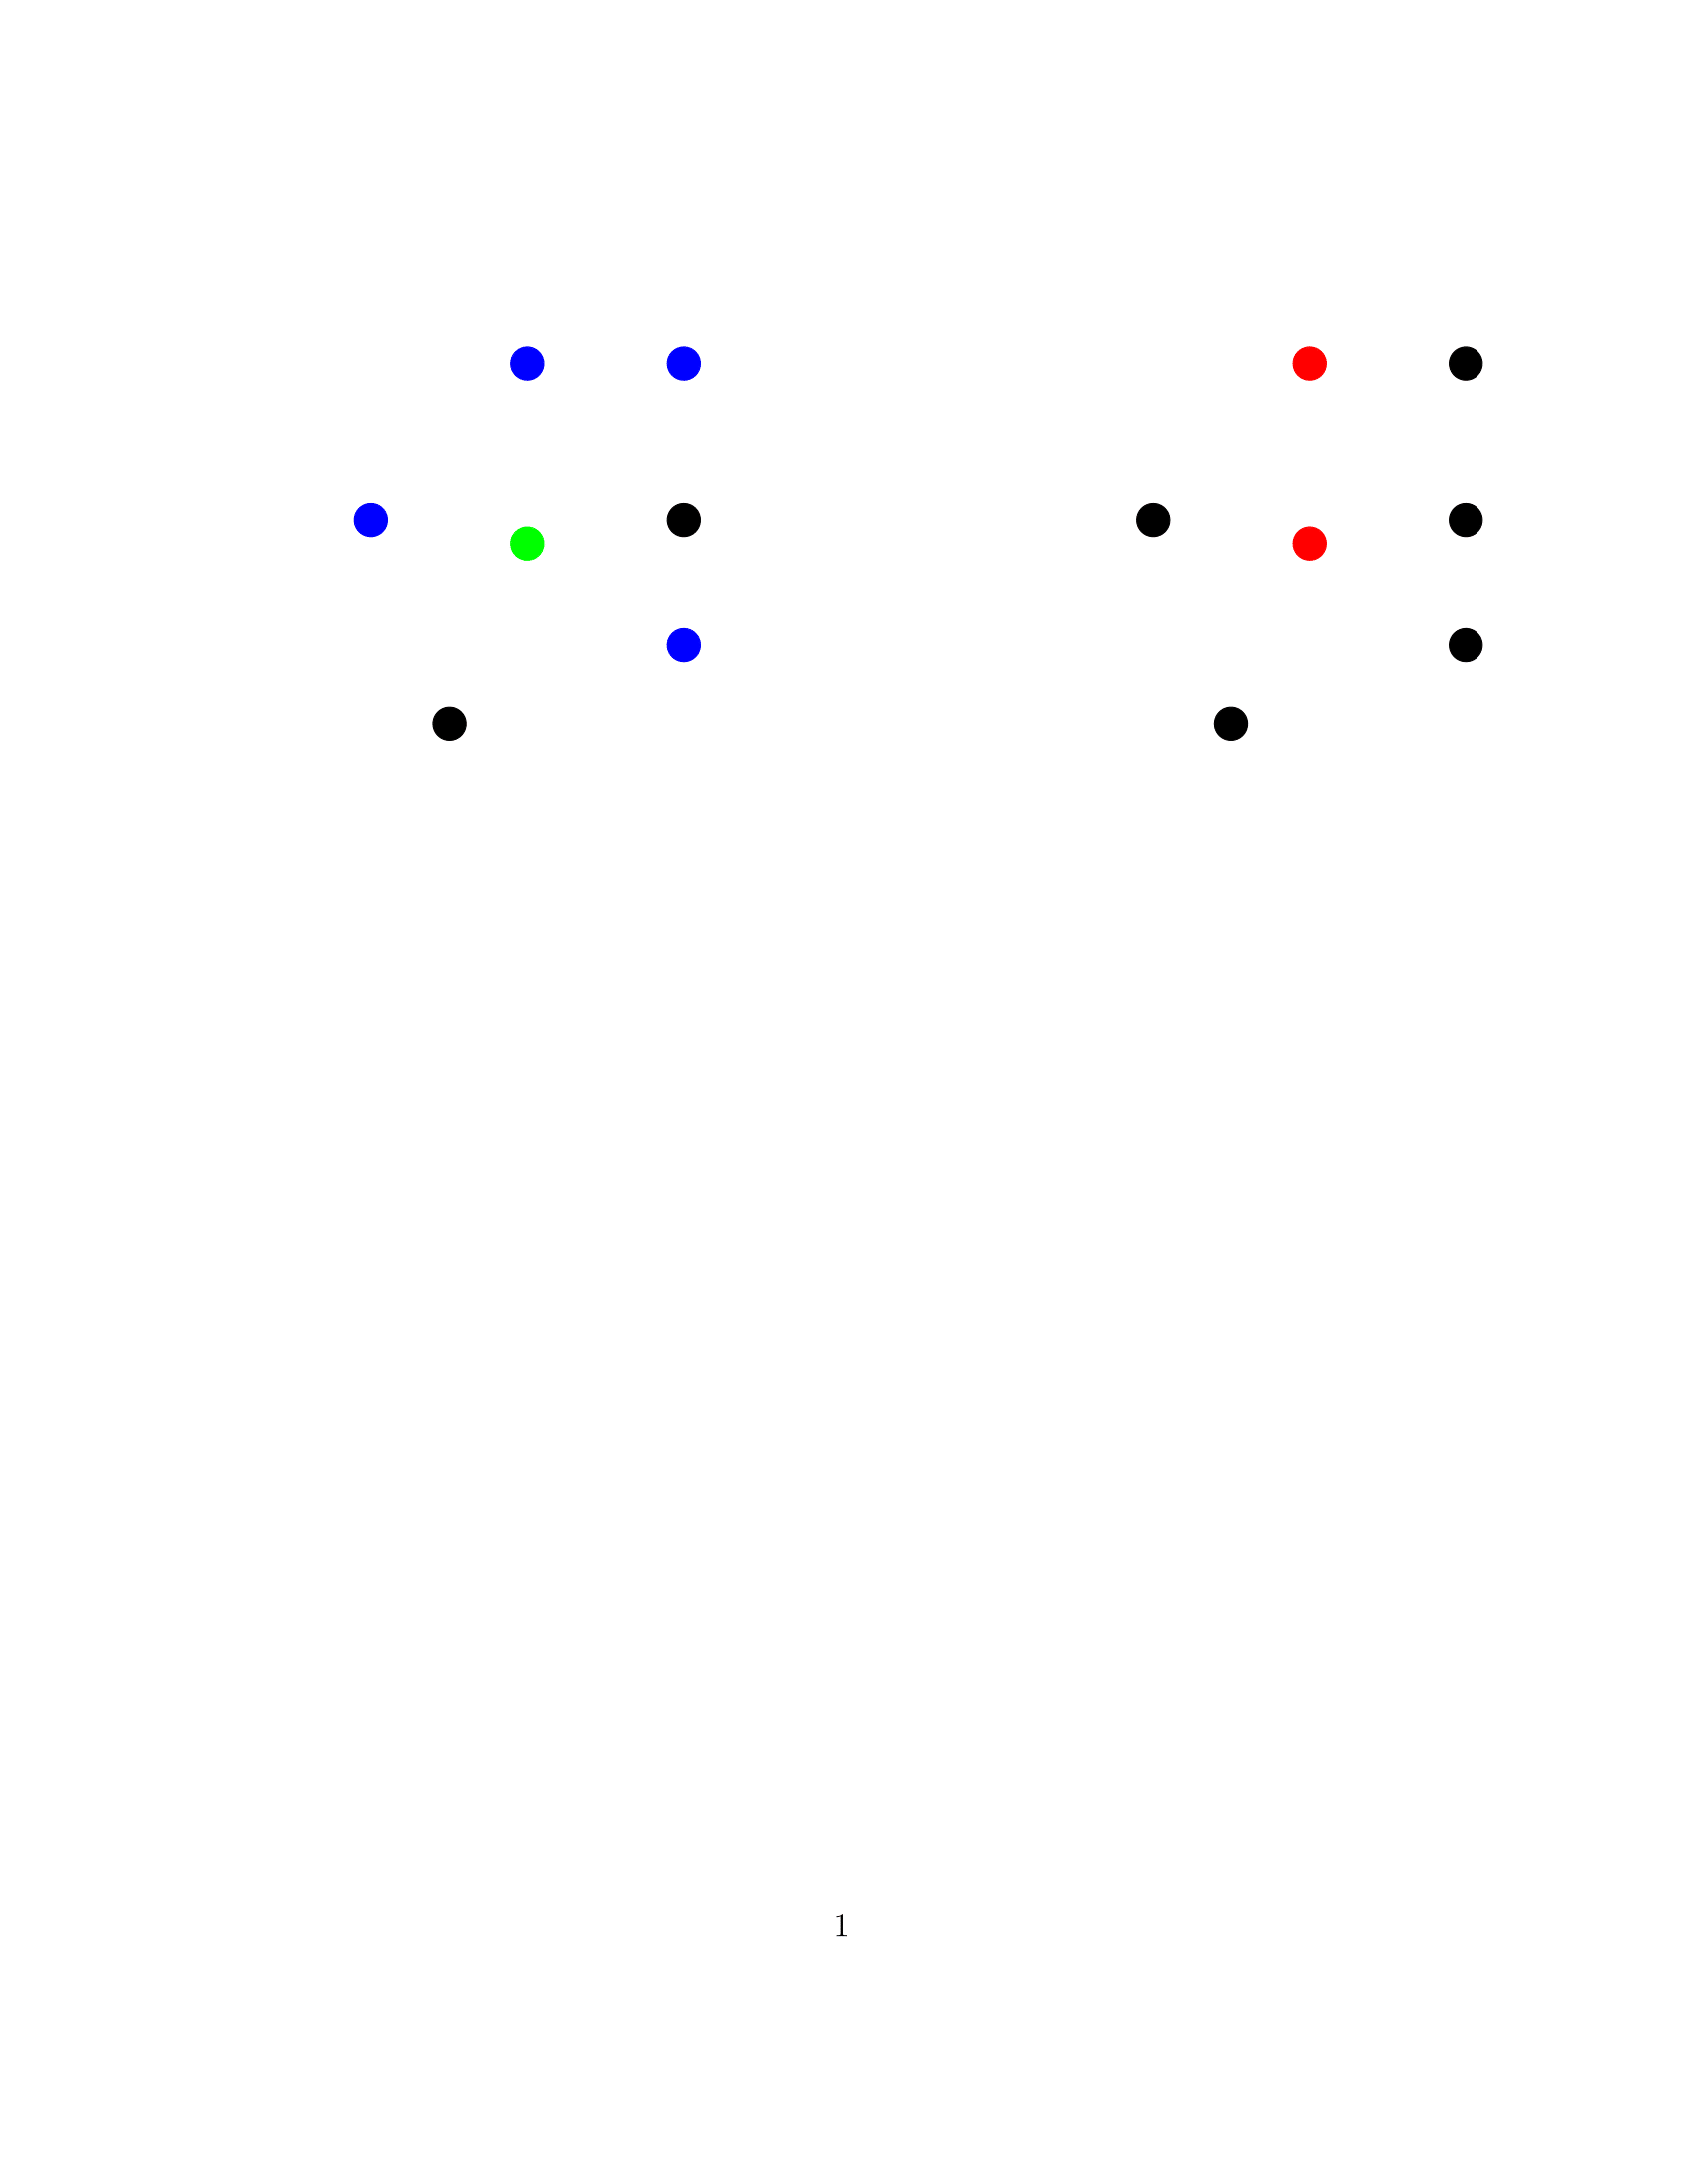
\includegraphics[scale=0.15]{figures/gammaAlg/gammaAlgo-4.png}}
	\only<6>{\centering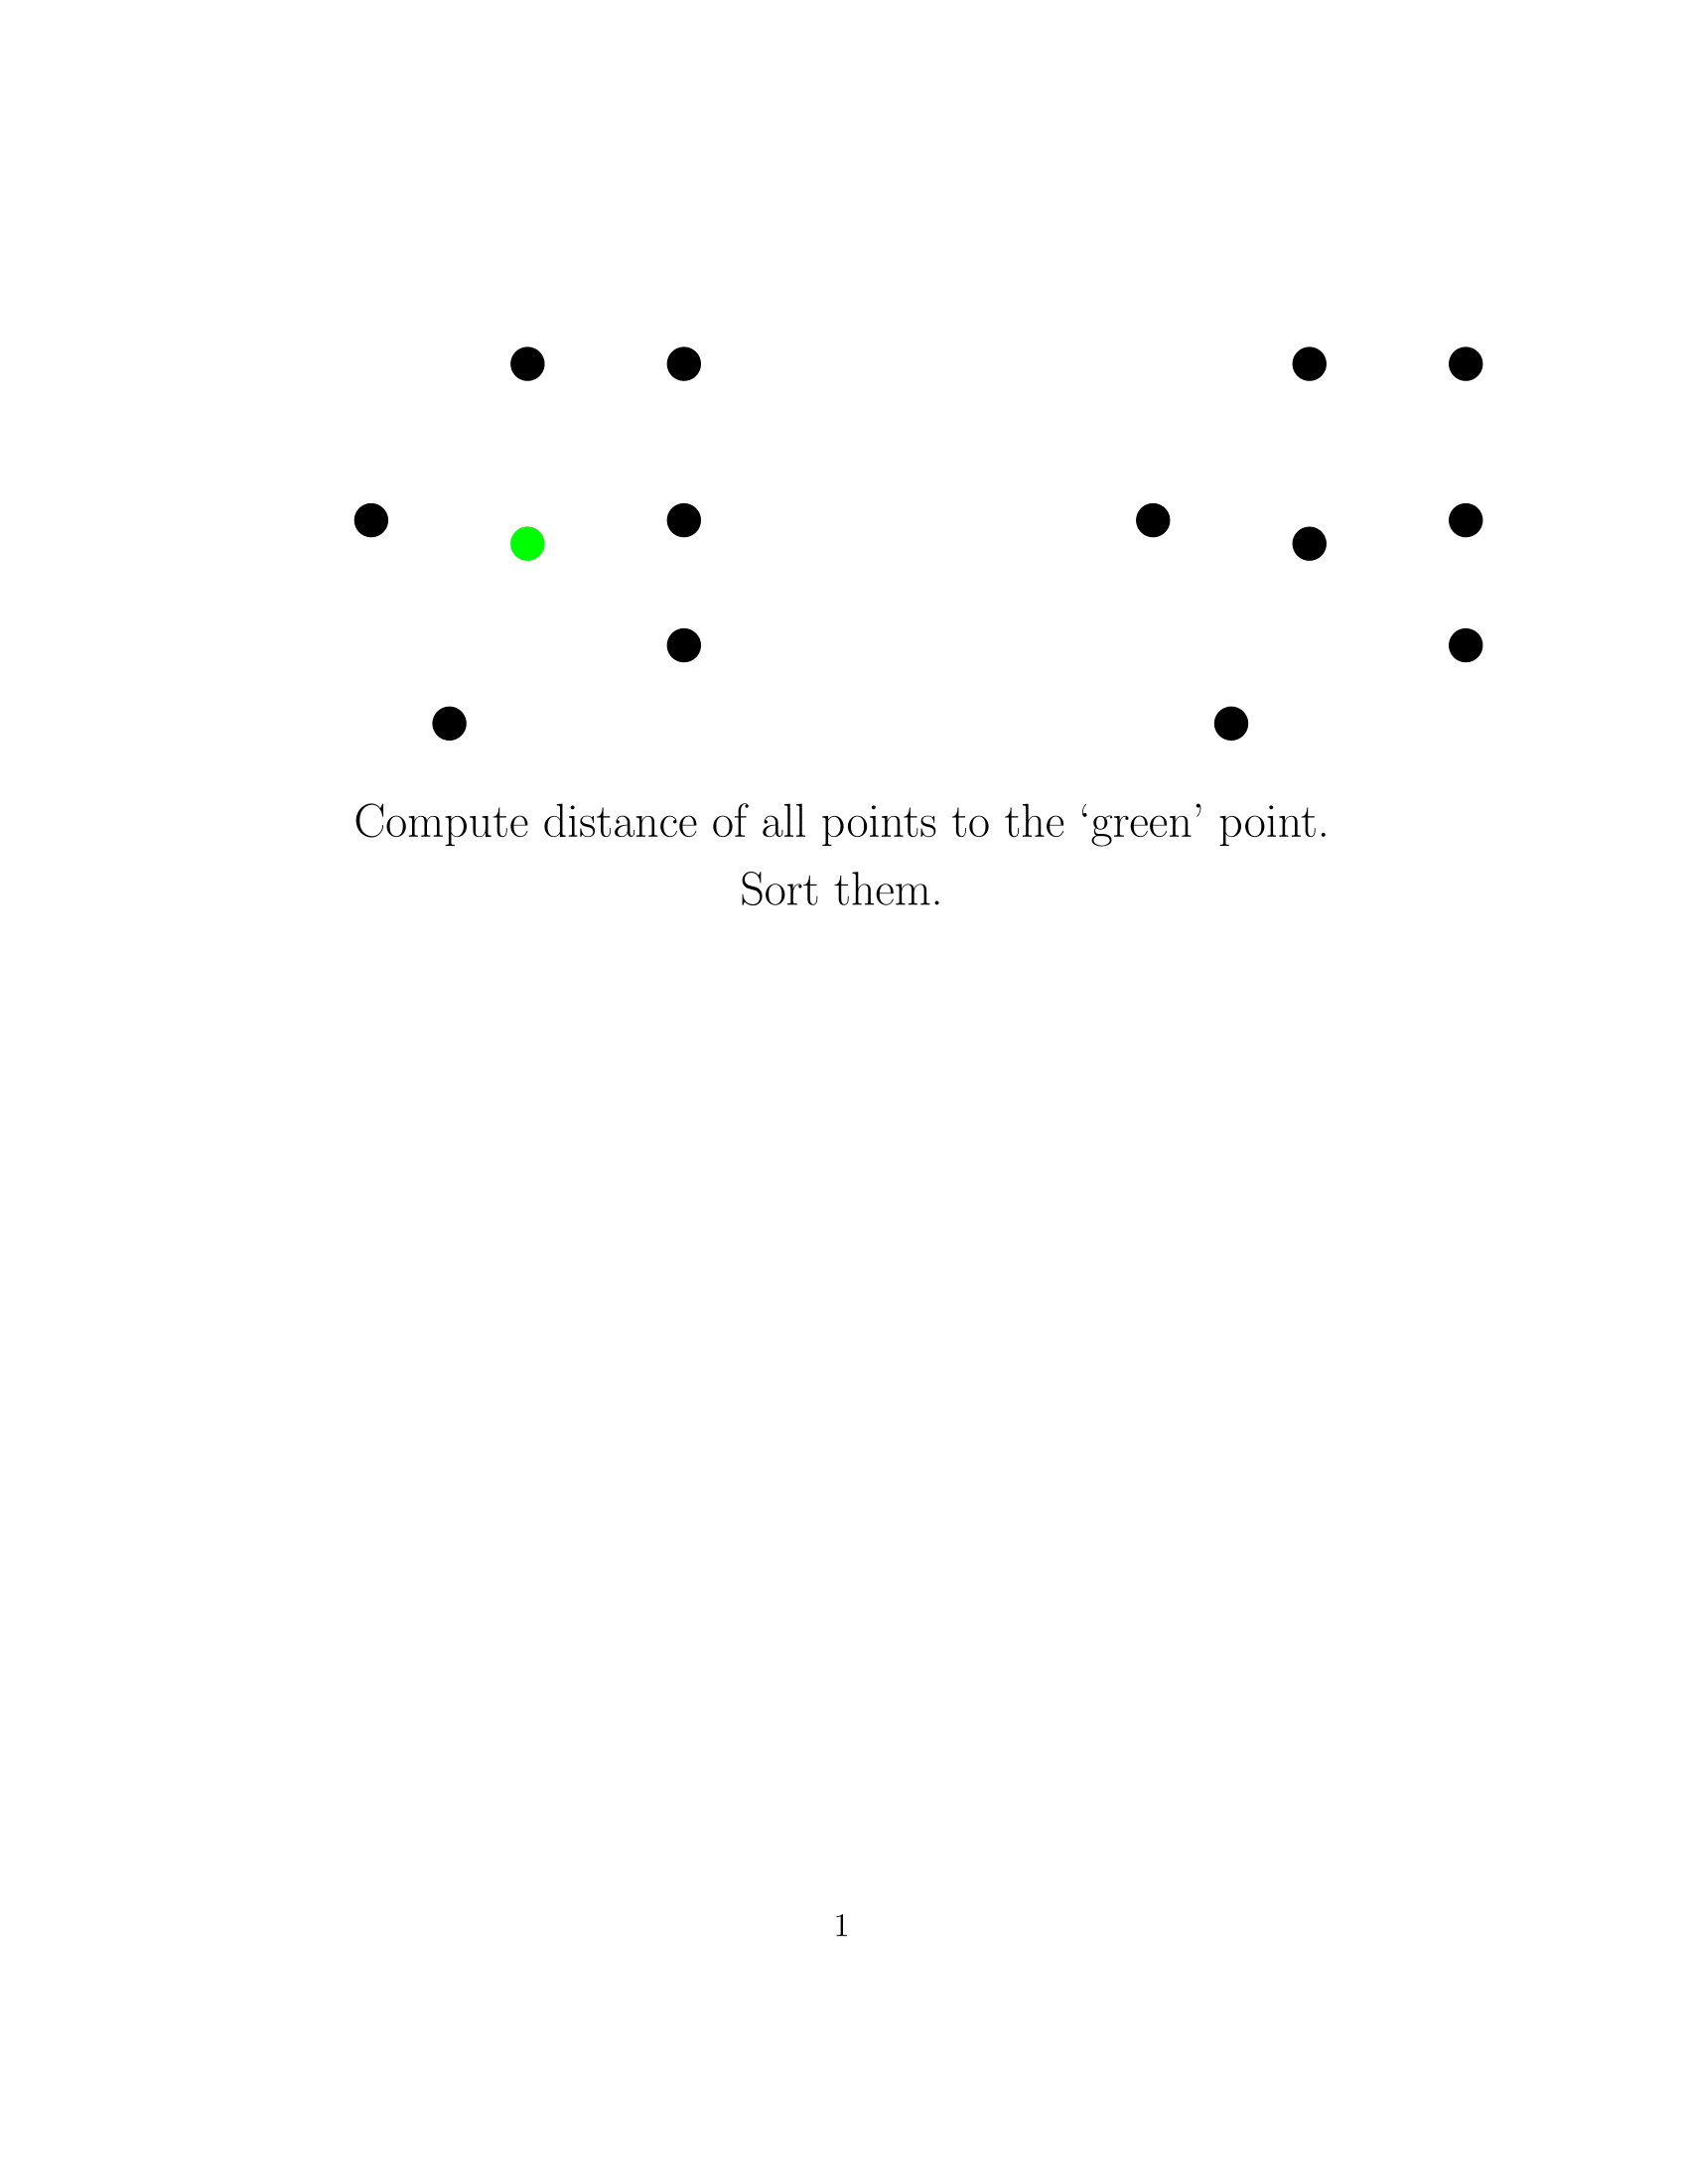
\includegraphics[scale=0.15]{figures/gammaAlg/gammaAlgo-5.png}}
	\only<7>{\centering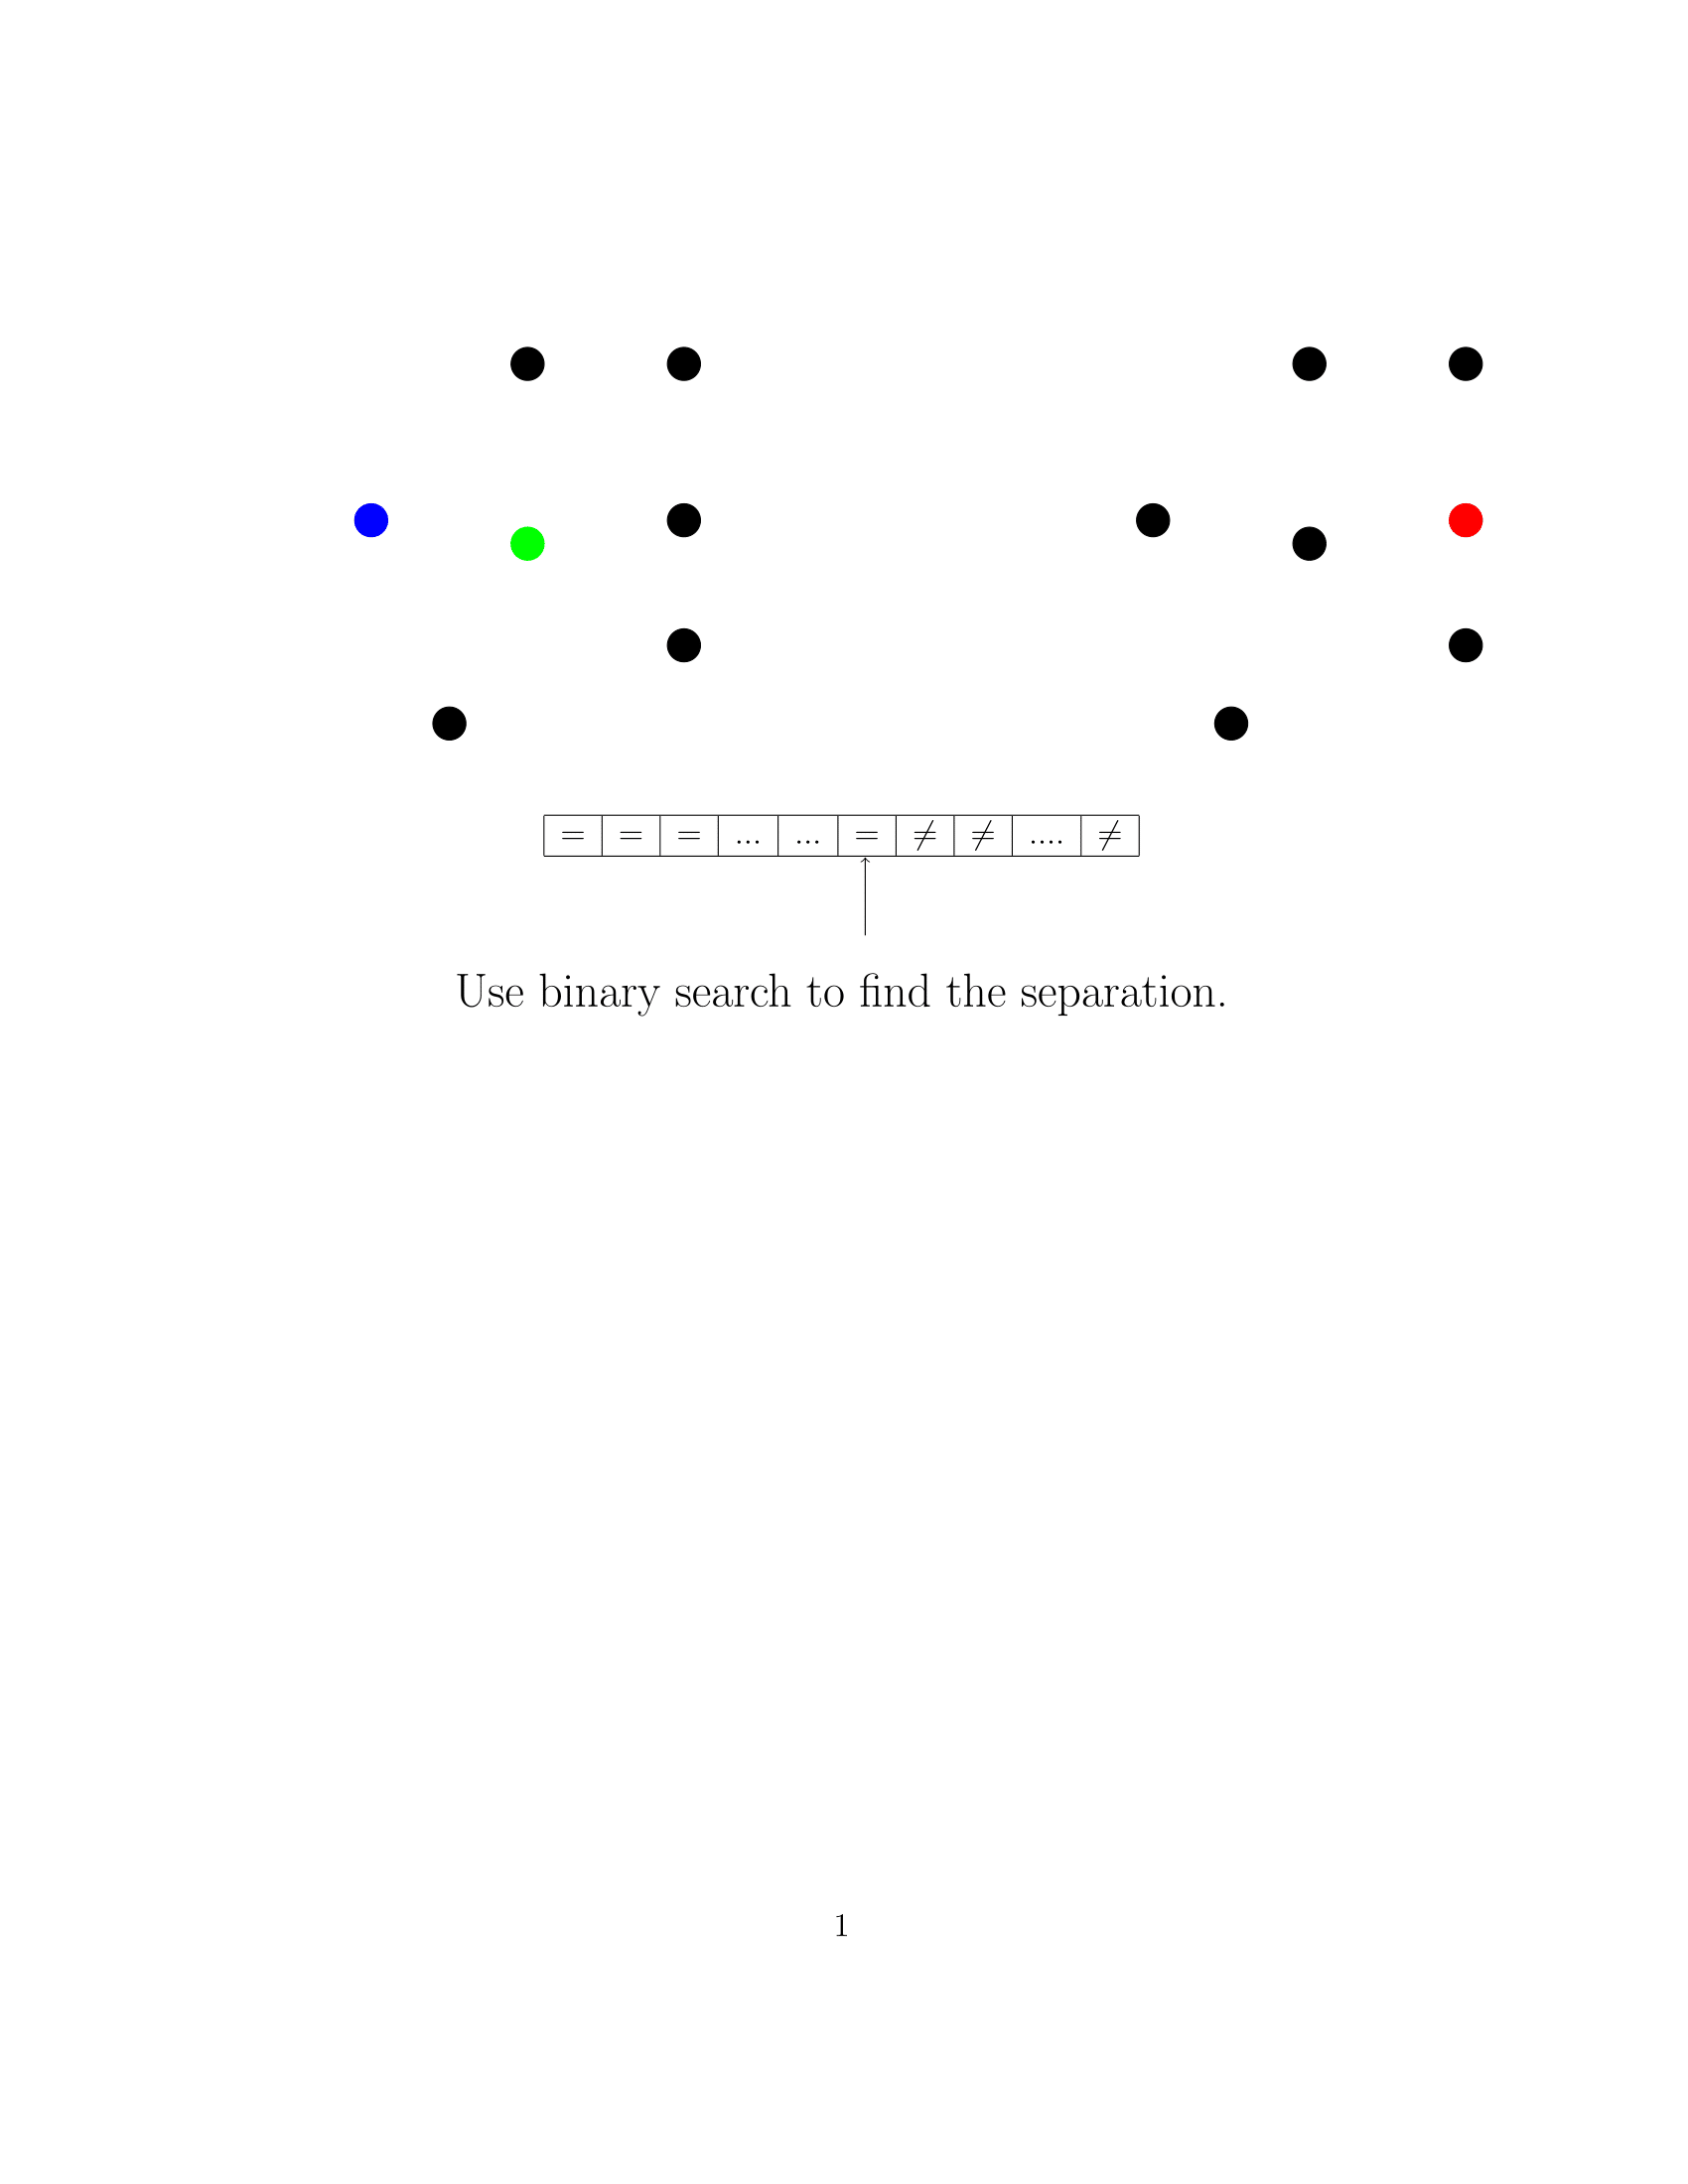
\includegraphics[scale=0.15]{figures/gammaAlg/gammaAlgo-6.png}}
	\only<8>{\centering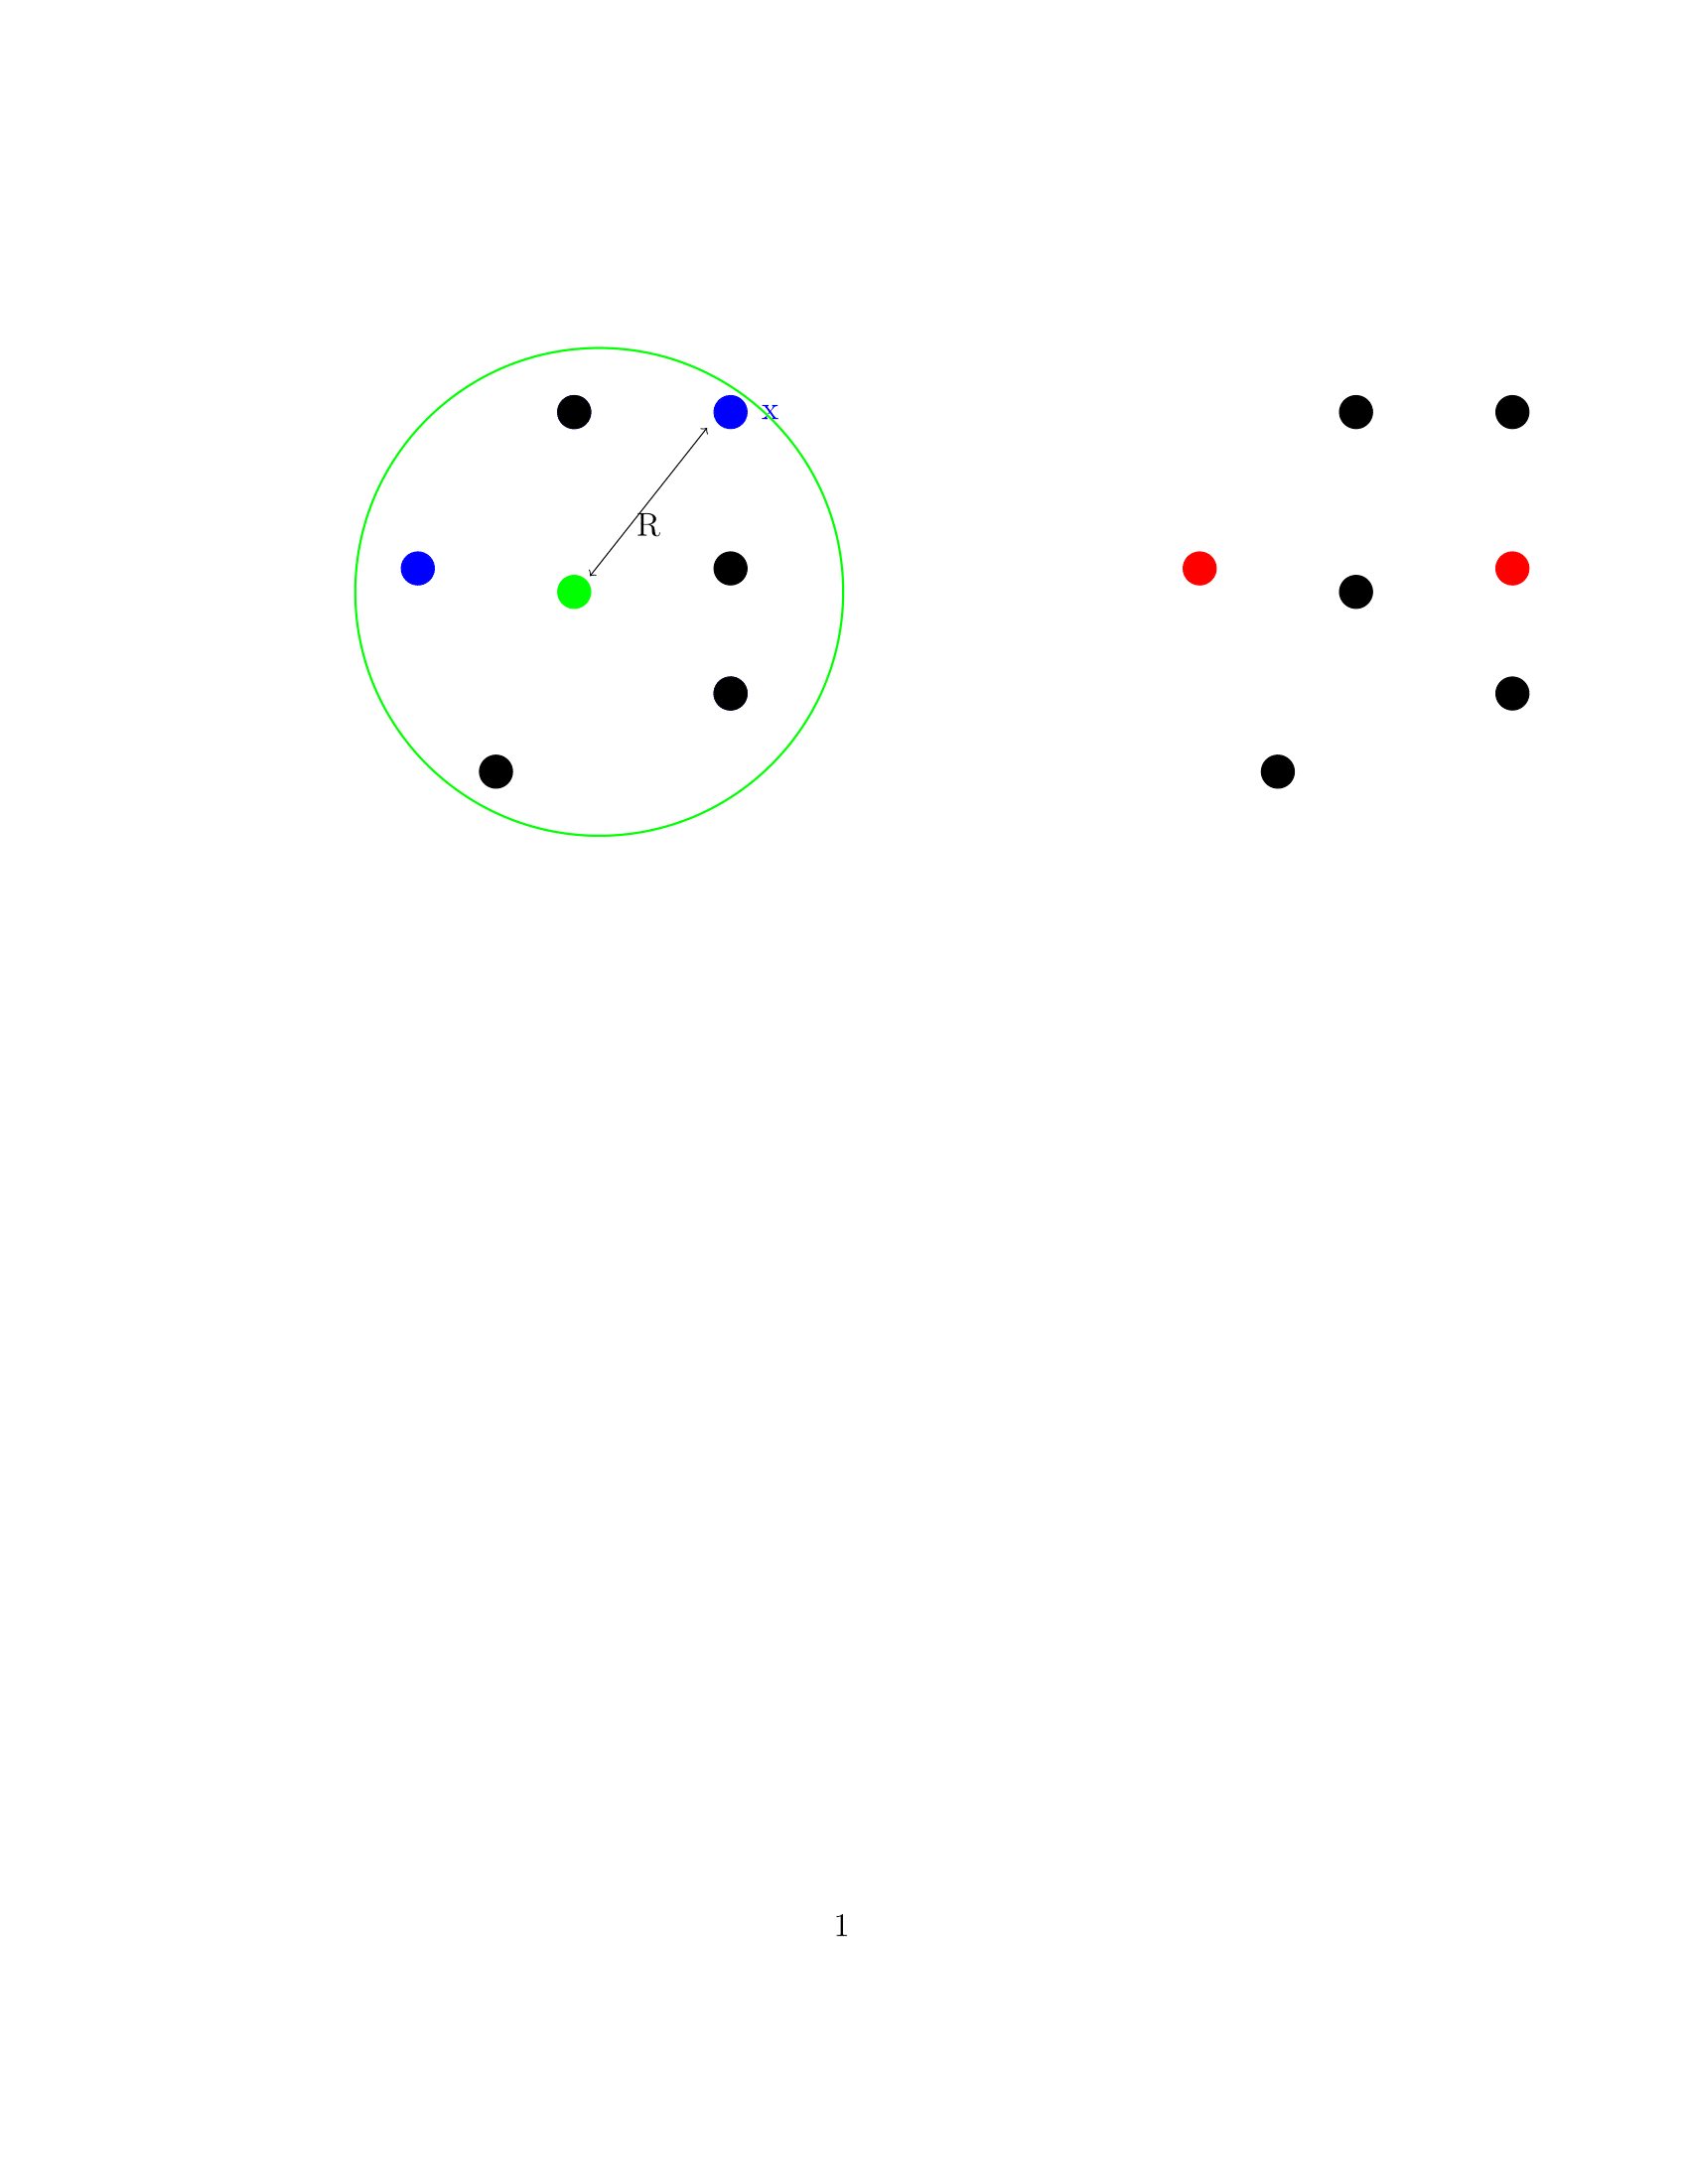
\includegraphics[scale=0.15]{figures/gammaAlg/gammaAlgo-7.png}}
	\only<9>{\centering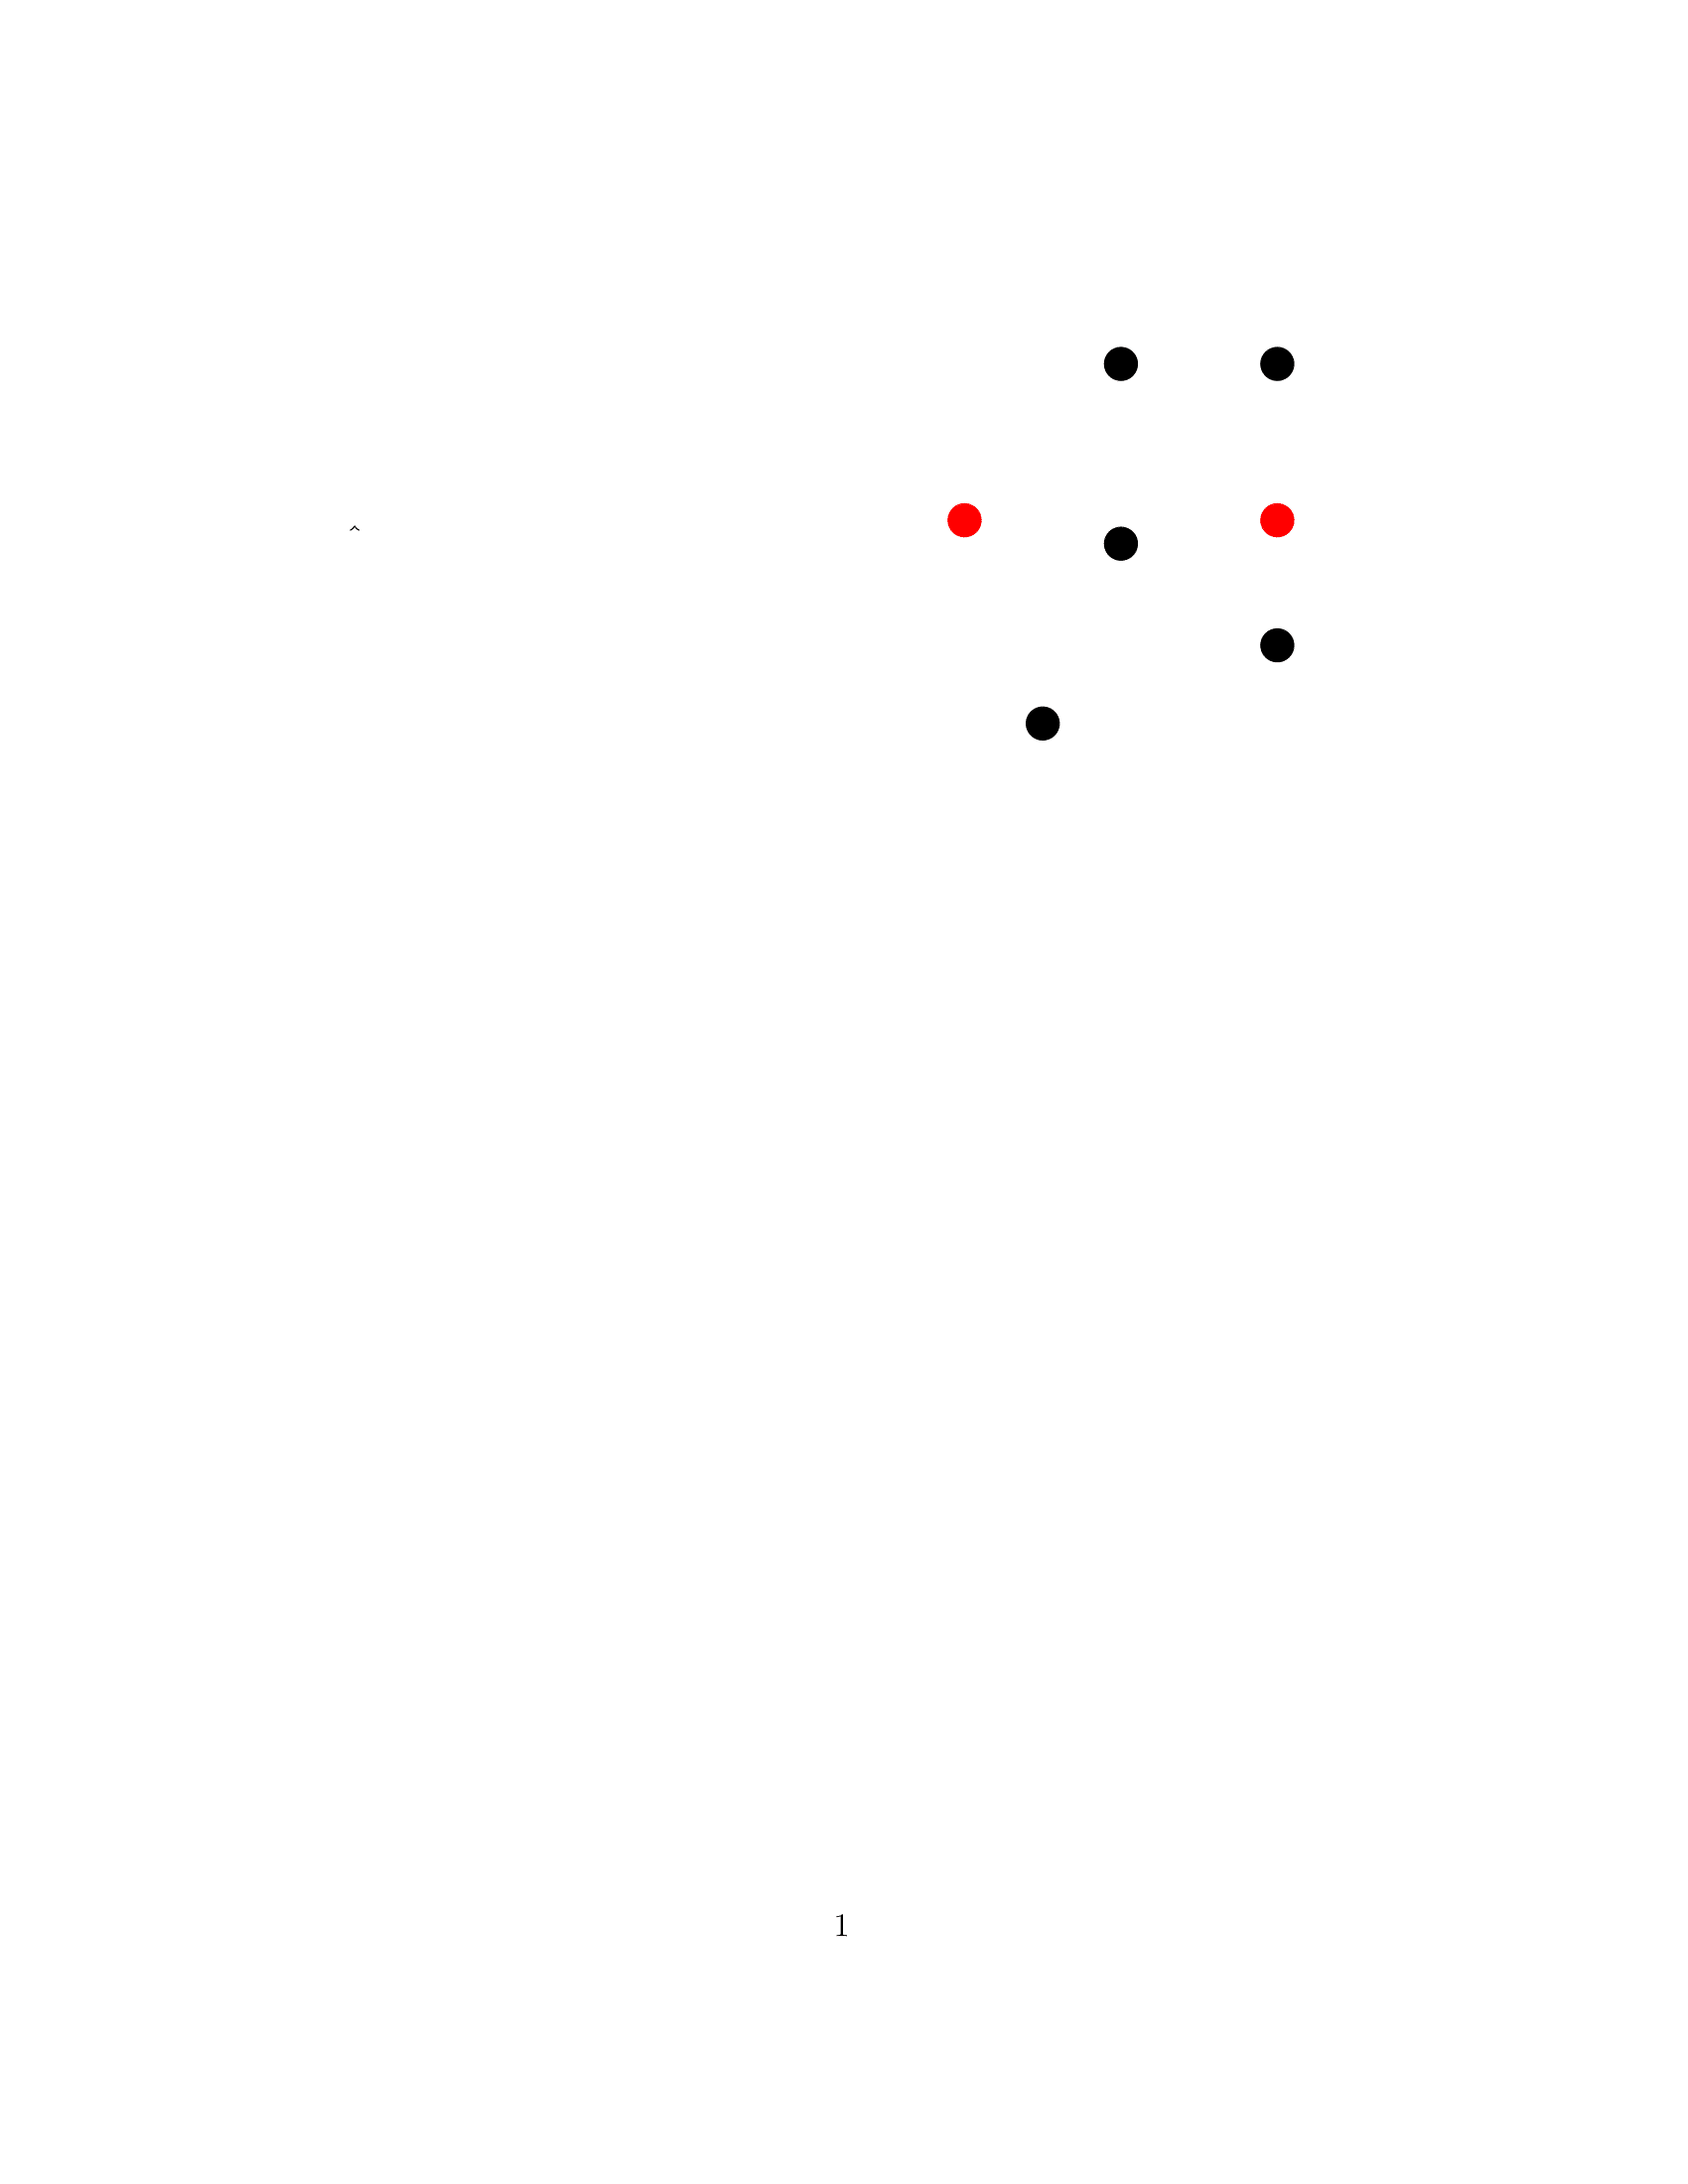
\includegraphics[scale=0.15]{figures/gammaAlg/gammaAlgo-8.png}}
\end{frame}
      
\begin{frame}{Lower Bound}
	Euclidean $k$-means is NP-hard even when the optimal solution satisfies the $\gamma$-margin property for $\gamma < 1.84$
	\vspace{0.3cm} 
	\begin{itemize}
		\item Reduction from Exact Cover by 3-Sets ($X3C$).
    	\vspace{0.3cm}\item Hardness for $k = \theta(n^{\epsilon})$
	\end{itemize}
	\pause
	\vspace{0.7cm}Small number of queries
	\vspace{0.3cm}
	\begin{itemize}	
		\item NP-hard with $O(\log n)$ queries for $\gamma < 1.84$
	\end{itemize}	    
\end{frame}

\begin{frame}{Summary}
  \begin{itemize}
    
    \item Interactive model for clustering
    \vspace{0.5cm}
    \item An efficient algorithm to find the ``true'' clustering
    \vspace{0.5cm}
    \item An NP-hard problem became tractable using few queries
  \end{itemize}
\end{frame}

\begin{frame}{Future work}
	Various avenues for future work.
	\begin{itemize}
		\vspace{0.9cm}\item Computational complexity 
		\vspace{0.9cm}{\color{lb} \MyCitem Under-specificity}
	\end{itemize}
\end{frame}

\begin{frame}{Dealing with computational complexity}
	Clusterability notion should be
	\begin{itemize}
		\vspace{0.3cm}\item Realizable
		\vspace{0.3cm}\item Efficient
		\vspace{0.3cm}\item Verifiable
		\vspace{0.3cm}\item Explanation of popular methods
	\end{itemize}
\end{frame}

\begin{frame}{Sparse noise against these metrics}
	Realizable?
	\begin{itemize}
		\vspace{0.3cm}\item Seems so !!
		\vspace{0.3cm}\item Can we find datasets that satisfy our criteria?
	\end{itemize}
	
	\vspace{1cm}Convergence of popular heuristics?
\end{frame}

\begin{frame}{Clusterability notion}
	\vspace{1cm}Efficient?
	\begin{itemize}
		\vspace{0.4cm}\item Efficiently represent all solutions 
		\vspace{0.4cm}\item Find any (not all) nice solutions?
		\vspace{0.4cm}\item Objective-based clustering in the presence of noise?
	\end{itemize}
\end{frame}


\begin{frame}{Future work}
	Various avenues for future work.
	\begin{itemize}
		\vspace{0.9cm}{\color{lb} \MyCitem Computational complexity }
		\vspace{0.9cm}\item Under-specificity
	\end{itemize}
\end{frame}

\begin{frame}{Dealing with under-specificity}
    Realistic?
	\begin{itemize}
		\vspace{0.3cm}\item user mistakes?
		\vspace{0.4cm}\item user abstensions?
		\vspace{0.4cm}\item Handle noisy points where there is no clear cluster membership?
		\vspace{0.4cm}\item Implement on a dataset?
	\end{itemize}
\end{frame}

\begin{frame}{Dealing with under-specificity}
	\vspace{1cm}Efficient?
	\begin{itemize}
		\vspace{0.4cm}\item Improve queries while relaxing other parameters?
		\vspace{0.4cm}\item Recovery from tree?
	\end{itemize}
\end{frame}

\begin{frame}
    \Huge{\centerline{Thank You!}}
\end{frame}

\begin{frame}{Notions of clusterability}
	
	{\color{blue} Weak-deletion stability}\\
	\vspace{0.5cm}$$OPT^{(i \leftarrow j)} > (1 + \alpha)OPT$$
	$k$-median and $k$-means:
	\begin{itemize}
		\item finds $(1+\epsilon)$-approximation.
		\item Runs in $O(n^{\frac{1}{\alpha \epsilon}} k^{\frac{1}{\epsilon}})$ and $O(n^3 (k\log n)^{poly(\frac{1}{\alpha}, \frac{1}{\epsilon})})$ respectively
	\end{itemize}
	
	\vspace{0.5cm}\alert{Issues}\\
	\begin{itemize}
	\item $\frac{1}{\alpha} > k \frac{AvgDis}{d_{min}}$. 
	\item For ``most" clusters:\\ $d(x, ci) >= 0.5 \alpha \log(k) AvgDis$
	\end{itemize}
\end{frame}

\begin{frame}{Notions of clusterability}
	
	{\color{blue} Additive perturbation robustness}\\
	$$\forall x, y  \hspace{0.4in}|d(x, y) - d'(x, y)| \le \epsilon\vspace{0.5cm}$$

	Optimal solution doesn't change under small additive perturbations.\\
	
	\vspace{1cm}\alert{Issues}\\
	\begin{itemize}
		\item Runtime exponential in $k$. $O(kn^{\frac{k}{\epsilon^2}})$
	\end{itemize}
\end{frame}

\begin{frame}{Notions of clusterability}
	
	{\color{blue} Center separation}\\
	$$ d(c_i, c_j) > \lambda r(\mc C) $$

	covered by k well-separated set of balls \\
	
	\vspace{0.5cm}{\color{blue}Robustified version} - clustering on the nice set should be the same.\\
	
	\vspace{1cm}\alert{Strong clusterability requirement}\\
	\begin{itemize}
		\item 	For 5\% noise, their algorithm is able to obtain a robustified version of 2-median if unit balls are separated by distance 10.

	\end{itemize}
\end{frame}

\begin{frame}{Hardness proof}
	$U = \{1, \ldots, 3m\}$ \\ 
	$\mc S = \{S_1, \ldots, S_l\}$ \\
	$S_i \subseteq U$ and $|S_i| = 3$\\ 
	
	\vspace{1cm} Does there exist $m$ elements in $\mc S$ such that their union is $U$? 	
\end{frame}

\begin{frame}{Hardness proof contd $\ldots$}
	\begin{align*}
	&h = \sqrt{5}, d = \sqrt{6}, \epsilon = \frac{1}{w^2}, \lambda = \frac{2}{\sqrt{3}}h, k = (l-1)3m + l(3m+2)\\
	& L_1 = (6m+3)wl, L_2 = 3m(l-1)w, L = L_1 + L_2 - m\alpha, \alpha = \frac{d}{w}-\frac{1}{2w^3}
	\end{align*}
	
	\begin{figure}
		\begin{subfigure}{.5\textwidth}
		\includegraphics[trim= 100 700 100 100,scale=0.7]{figures/lowerBdFig.pdf}
		\end{subfigure}
		\begin{subfigure}{.5\textwidth}
		\includegraphics[trim=300 400 300 100, scale=0.5]{figures/ZFig.pdf}
		\end{subfigure}
	\end{figure}
	
	
\end{frame}


%----------------------------------------
%        Figure Samples
%----------------------------------------

% All of the following is optional and typically not needed. 
\appendix
\section<presentation>*{\appendixname}
\subsection<presentation>*{For Further Reading}

%\begin{frame}[allowframebreaks]
  %\frametitle<presentation>{For Further Reading}
   % 
  %\begin{thebibliography}{10}
    
  %\beamertemplatebookbibitems
  % Start with overview books.

  %\bibitem{Author1990}
   % A.~Author.
    %\newblock {\em Handbook of Everything}.
    %\newblock Some Press, 1990.
 
    
  %\beamertemplatearticlebibitems
  % Followed by interesting articles. Keep the list short. 

  %\bibitem{Someone2000}
   % S.~Someone.
    %\newblock On this and that.
    %\newblock {\em Journal of This and That}, 2(1):50--100,
    %2000.
  %\end{thebibliography}
%\end{frame}

\end{document}


